\documentclass[xcolor={dvipsnames}]{beamer}
\usepackage{amsmath}
% \usepackage{beamerthemesplit} // Activate for custom appearance
\usepackage{hyperref}
\usepackage{ragged2e}
\input xy 
\xyoption{all}
\usepackage{color}

\font\domino=domino
\def\die#1{{\domino#1}}

\title{Ensemble Methods (Part I)\\
Bagging and Random Forests}
\author{Schwartz}
\date{\today}

\begin{document}

\frame{\titlepage}




\frame
{
 \frametitle{Trees!}
 
{
\fontfamily{<familyname>}\selectfont
\begin{quote}
\tiny
\justify
A recent study published in the Proceedings of the National Academy of Sciences estimates that there are somewhere between 40,000 to 50,000 unique tree species in the American neotropics and Indo-Pacific tropics, respectively, and that tropical Africa includes an additional approximately 10,000 species. This amount of tree diversity far outpaces tree diversity in temperate regions. For example, temperate forests in Europe have only 124 unique tree species and there are only approximately 1,000 tree species in North America.  
Another recent study published in Nature estimates that there are 3.04 trillion trees on earth -- 422 per person -- and that 45\% of the trees are in the tropics.  Tropical forests make up 2\% of the earth's landmass. By area then, tropical jungles produce tree diversity at a rate of 5000:1 and tree density at a rate of 40:1 compared the rest of the earth's dry landmasses. 
\end{quote}
}

\begin{figure}
\centering
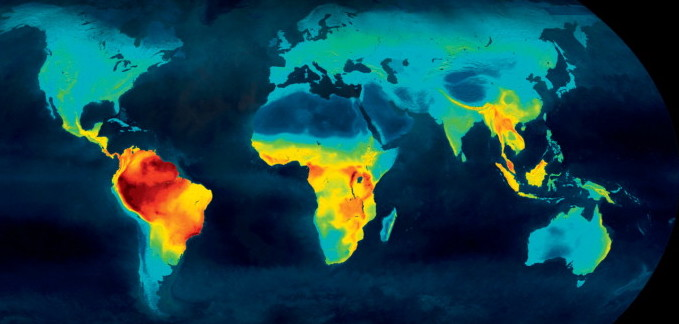
\includegraphics[width=3.65in]{stuffs/biodiversity.jpg}
\end{figure}

}

\frame
{
 \frametitle{Objectives}
\begin{itemize}
\item<1-> What is \emph{Bagging}?
\begin{itemize}
\item<2-> How do you do it?
\begin{itemize}
\item<3-> Why is it good?
\end{itemize}
\end{itemize}
\item[]
\item<4-> What are \emph{Random Forests}?
\begin{itemize}
\item<5-> How do you make them?
\begin{itemize}
\item<6-> Why might they be an improvement over bagging?
\end{itemize}
\end{itemize}
\item[]
\item<7-> What is ``out of bag error'' (OOB) relative to $K$-folds?
\item[] 
\item<8-> How can one interpret variables in tree ensembles?
%\item<9-> Be able to implement tree-ensemble methods

%%%\item<9->[] \textcolor{red}{This will be a trial by fire test of what you know about trees}

%GET someone to the front to write these on the board.
% Now this is a review that we do at the beginning of class:

% interpretability
% makes very flexible interactions: highly non linear okay 

% can classify and predict: what's the difference

% mixed feature types -
% missing values (not in python, but can convert to indicator, or can just decide later down tree)
% no preprocessing 
% can start with *a lot* of features no prob

% not so good? yeah, probably

% expensive to train? yeah, probably
% bias/variance tradeoff in trees?
% parameters: 
%      number of leaves 
%      max depth 
%      min number of samples per leaf
%      min number of samples to split
%      build and prune back to protect from overfitting?
%      consider number of leaves T as a tuning parameter?

 \end{itemize}

}



\frame
{
 \frametitle{Single Predictors/Estimators}

\begin{itemize}
\item<1-> \textcolor{ForestGreen}{A single tree is pretty great! }
\item<2-> \textcolor{ForestGreen}{Well, it's not that good, actually }
\item[]<3-> \textcolor{ForestGreen}{What could be wrong with it?}
\begin{itemize}
\item[]<4-> \textcolor{Sepia}{Biased?}
\item[]<4-> \textcolor{Sepia}{High variance?} 
\item[]<5-> \textcolor{Sepia}{\emph{How so with trees?}} 
% build and prune back to keep from overfitting?
% maybe use cross validation to select tree depth
\end{itemize}
\item[]<6-> Do we think a prediction from a single tree is good? 
% trees maybe aren't actually that good
% extrapolation 


%\item[]
%\item<7-> What if we had a lot of prediction trees\\ \onslide<8->{\emph{\textcolor{red}{and averaged or majority voted with their predictions?}}}
\end{itemize}
}



\frame
{
 \frametitle{Ensemble Challenge}
THIS IS GARBAGE -- need a much better presentation...


\begin{figure}
\centering
Suppose you are trying to predict the election...\\${}$\\
You have 5 expert opinions, each with a 70\% chance of being right,\\
and each expert pick is \emph{independent} of the other expert picks.\\${}$\\
How could you leverage expert picks to improve accuracy \\
and how often would you be right?

% binom(x>=3, n=5,p=.7)
% from scipy import stats
% 1 - stats.binom.cdf(2,n=5,p=.7)
% 1 - stats.binom.cdf(51,n=101,p=.7)
% 1 - stats.binom.cdf(26,n=53,p=.7) -> answer is 55

\vspace{.35in}

\color{blue}
\onslide<2->{How many independent predictors would you need \\
to have a 99.9\% of being correct?}\\${}$\\

\color{red}
\onslide<3->{\textcolor{white}{$<$} \texttt{1 - stats.binom.cdf(26,n=53,p=.7)} $< .001$\\
$<$ \texttt{1 - stats.binom.cdf(27,n=55,p=.7)} \textcolor{white}{$< .001$}}


\end{figure}
}



\frame
{
\frametitle{Averaging Multiple Predictors/Estimators}

\begin{itemize}
\item<1-> \textcolor{blue}{Let $\hat f^{(j)}({\boldsymbol x}_0)$ be the $j^{th}$ predictor of outcome $f({\boldsymbol x}_0)$ constructed 
from a training set with features ${\boldsymbol x}^{(j)}$ and outcomes ${\boldsymbol Y}^{(j)}$}
\item[]
\item<1-> If each $\hat f^{(j)}({\boldsymbol x}_0)$ is an unbiased predictor of $f({\boldsymbol x}_0)$ then
$$\text{E}\left[\frac{1}{m} \sum_{j=1}^m \hat f^{(j)}({\boldsymbol x}_0)\right] = f({\boldsymbol x}_0)$$
\item[]<2-> \textcolor{red}{$\hat f^{(j)}({\boldsymbol x}_0)$ can be an unbiased predictor by being highly complex}
\item[]<3-> E.g., \textcolor{blue}{like an overfit tree!}
\item<4-> And if $\text{Var}\left[\hat f^{(j)}({\boldsymbol x}_0)\right] = \sigma^2$, then  
$\displaystyle \text{Var}\left[\frac{1}{m} \sum_{j=1}^m \hat f^{(j)}({\boldsymbol x}_0)\right] = \only<5->{\frac{\sigma^2}{m}}\text{?}$
\item[]<6-> \textcolor{red}{So even if $\hat f^{(j)}$ is a high variance predictor} \onslide<7->{\textcolor{blue}{the variance}}
\item[]<7-> \textcolor{blue}{of the \emph{averaged} predictor $\frac{1}{m} \sum_{j=1}^m \hat f^{(j)}$ decreases with $m$} 

\end{itemize}

}




\frame
{
\frametitle{What is happening?}
%%% accuracy of a decision tree? bias/variance? why is bagging

\begin{columns}
\begin{column}{.05\textwidth}
${}$
\end{column}
\begin{column}{.5\textwidth}
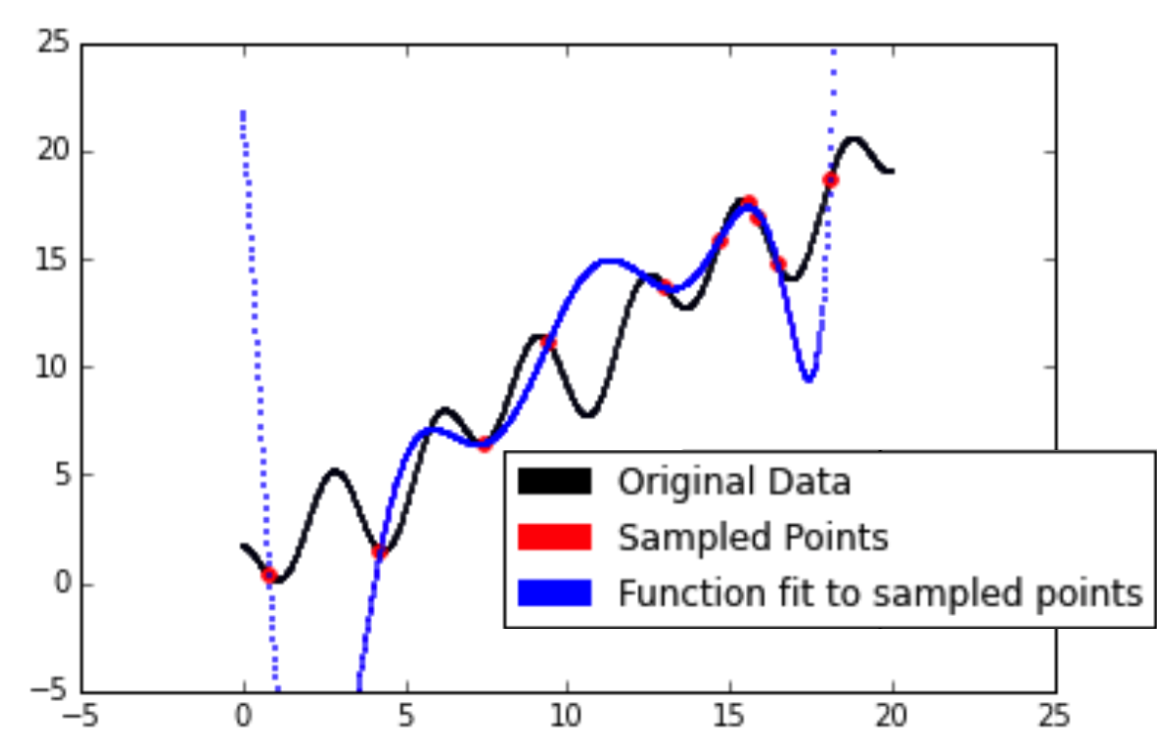
\includegraphics[width=2.1in]{stuffs/rfex3.png}

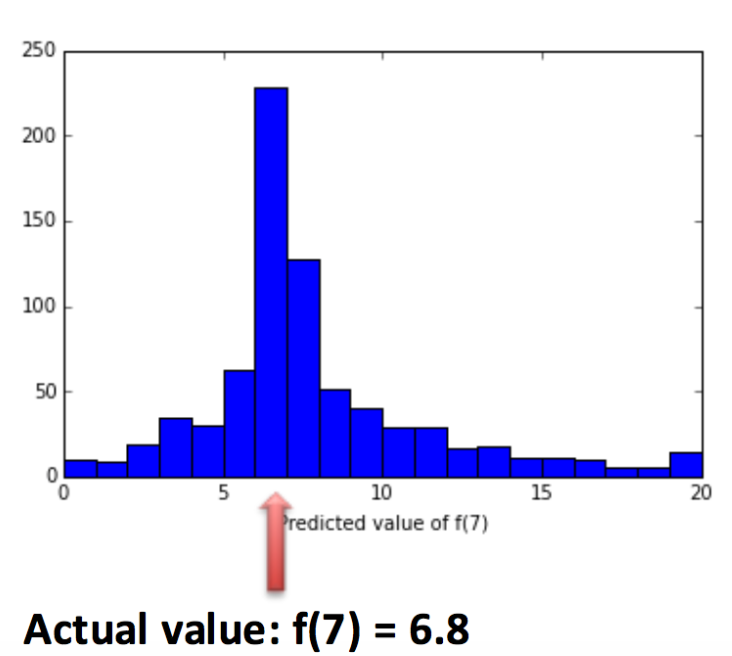
\includegraphics[width=2in]{stuffs/rfex2.png}
\end{column}
\begin{column}{.4\textwidth}
\raisebox{.14\height}{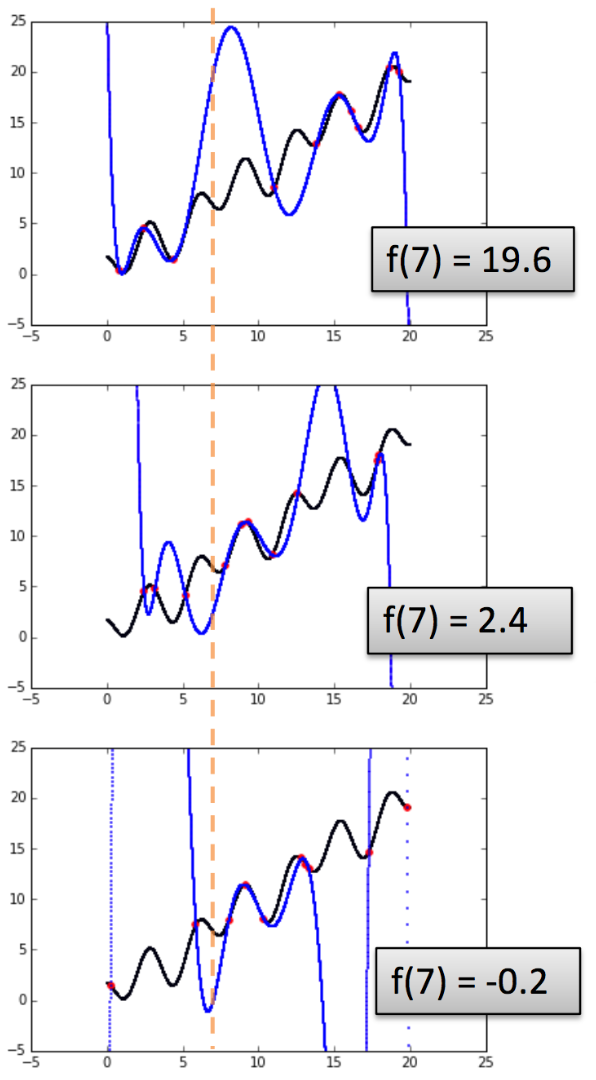
\includegraphics[height=2.73in]{stuffs/rfex4.png}}
\end{column}
\end{columns}

}




\frame
{
 \frametitle{Bootstrapping Aggregation (Bagging)}
\begin{itemize}
\item<1-> \textcolor{blue}{Let $\hat f^{(j)}({\boldsymbol x}_0)$ be a predictor of outcome $f({\boldsymbol x}_0)$ constructed 
from a training set with features ${\boldsymbol x}^{(j)}$ and outcomes ${\boldsymbol Y}^{(j)}$}
\item[]
\item<2-> \emph{Bagging} is simply predicting $f({\boldsymbol x}_0)$ with $\displaystyle \frac{1}{m} \sum_{j=1}^m \hat f^{(j)}({\boldsymbol x}_0)$
\item<2->[] \underline{an average of predictors made from bootstraped samples}
%\item<2->[]
%\item<3-> What are the $\hat f^{(j)}$'s? I.e, what are ${\boldsymbol x}^{(j)}$'s and ${\boldsymbol Y}^{(j)}$'s?
%\item[]<4-> \textcolor{red}{Bootstrapped samples from ${\boldsymbol x}$ and ${\boldsymbol Y}$}
\item<3->  \textcolor{red}{${\boldsymbol x}^{(j)}$ and ${\boldsymbol Y}^{(j)}$  is a \emph{bootstrapped} sample from ${\boldsymbol X}$ and ${\boldsymbol Y}$}
\item<3->  \textcolor{red}{$\hat f^{(j)}$ is the model fit on that bootstrapped training set}
\item<3->[] %I.e., bagging is the \emph{average} of a bunch of predictions
\item<4->[1.] Bootrapped trees provides unbiased, high variance predictors$^*$  
\item<5->[2.] Averaged estimators are lower variance than single predictors 
\item<6->[3.] Averaged predictors are still unbiased 
\item<7->[4.] Bootrapping explores the ``data set''/``predictors'' space:
then uses the average of predictors we might see under sampling
\item[]
\item<8->[$^*$]\emph{Bagging is a general ensemble procedure often used with trees}
\end{itemize}
}



\frame
{
\frametitle{``Out of Bag'' (OOB) testing error}
\begin{itemize}
\item \textcolor{blue}{Let ${\boldsymbol x}_0^{(j)}$ and ${\boldsymbol Y}_0^{(j)}$ be the features and outcomes not in ${\boldsymbol x}^{(j)}$}
\item<2-> OOB  prediction error is calculated from 
\item[]<2-> $${\boldsymbol Y}_0^{(j)} \;\text{ vs }\; \hat f^{(j)}\left({\boldsymbol x}_0^{(j)}\right)$$

i.e.,  actual ${\boldsymbol Y}_0^{(j)}$ versus prediction $\hat {\boldsymbol Y}_0^{(j)}$ from $\hat f^{(j)}\left({\boldsymbol x}_0^{(j)}\right)$
\end{itemize}
\onslide<3->{\noindent\makebox[\linewidth]{\rule{\paperwidth}{0.4pt}}}
\begin{itemize}
\item<3->[]
\begin{tabular}{c|cccccccccc}
%&\multicolumn{10}{c}{${\boldsymbol Y}_0^{(j)}$}\\
${(j)}$&$Y_1$&$Y_2$&$Y_3$&$Y_4$&$Y_5$&$Y_6$&$Y_7$&$Y_8$&$Y_9$&$\cdots$\\
${(1)}$&$\blacksquare$&$\blacksquare$&$\blacksquare$&$\square$&$\square$&$\blacksquare$&$\blacksquare$&$\square$&$\blacksquare$&\\
${(2)}$&$\square$&$\square$&$\blacksquare$&$\blacksquare$&$\blacksquare$&$\square$&$\blacksquare$&$\blacksquare$&$\blacksquare$&\\
${(3)}$&$\blacksquare$&$\square$&$\blacksquare$&$\blacksquare$&$\blacksquare$&$\square$&$\blacksquare$&$\square$&$\blacksquare$&\\
\vdots & \multicolumn{9}{c}{
\textcolor{gray}{\scriptsize Bootstrapped samples of size $n$ leave out $\sim \frac{1}{3}$ of the data}} \\
\end{tabular}



\item<4-> When the number of bootstrapped samples $ j = 1, \cdots m$ is large,
this closely approximates LOO test error estimation.
\item<5-> Parameter tuning can be done ``for free'' when model fitting 
\end{itemize}
\vspace{.075in}

}




\frame
{
\frametitle{But wait...}

$$\text{Var}\left[\sum_{j=1}^m \frac{1}{m} \hat f^{(j)}({\boldsymbol x}_0)\right] \not = \frac{\sigma^2}{m}$$

\begin{itemize}
\item<2-> Why?
\item[]<3-> 
%\vspace{-2.5em}
$$\text{Var}\left[X + Y\right] = \text{Var}\left[X\right] + \text{Var}\left[Y\right] + \textcolor{red}{2 \text{Cov}\left[X, Y\right]}$$
I.e.,
\begin{align*}
\text{Var}\left[\hat f^{(j)}({\boldsymbol x}_0) + \hat f^{(k)}({\boldsymbol x}_0)\right] = {}& \text{Var}\left[\hat f^{(j)}({\boldsymbol x}_0)\right] + \text{Var}\left[\hat f^{(k)}({\boldsymbol x}_0)\right] \\
{}& + \textcolor{red}{2 \text{Cov}\left[\hat f^{(j)}({\boldsymbol x}_0), \hat f^{(k)}({\boldsymbol x}_0)\right]}
\end{align*}

\item[]
\item[]<4->{\textcolor{gray}{
$\hat f^{(j)}$ and $\hat f^{(k)}$ are correlated: they're predicting the same thing
from bootstrapped samples ${\boldsymbol x}^{(j)}$/${\boldsymbol Y}^{(j)}$ \& 
${\boldsymbol x}^{(k)}$/${\boldsymbol Y}^{(k)}$ from ${\boldsymbol x}$/${\boldsymbol Y}$!}} 
 
\end{itemize}
}


\frame
{
\frametitle{How good is bagging?}

\begin{itemize}
\item<1-> If Cor$\left[\hat f^{(j)}, \hat f^{(k)}\right] = \rho$ for all $j$ and $k$
\item[]<2-> then
$$\text{Var}\left[\frac{1}{m}\sum_{j=1}^m \hat f^{(j)}({\boldsymbol x}_0)\right] = \rho \sigma^2 + (1 - \rho)\frac{\sigma^2}{m}$$

\item<3-> Only ``uncorrelated parts'' of $\hat f^{(j)}$ and $\hat f^{(k)}$ get ``CLT effect''
\item[]
\item<4-> So is there any way to get $\rho$ close to 0?
\end{itemize}
}






\frame
{
\frametitle{Decorrelating trees}

\begin{columns}
\begin{column}{.55\textwidth}

\vspace{.25em}
We might try to decorrelate any class of predictors $\hat f^{(j)}$ \\${}$\\

But let's focus on  
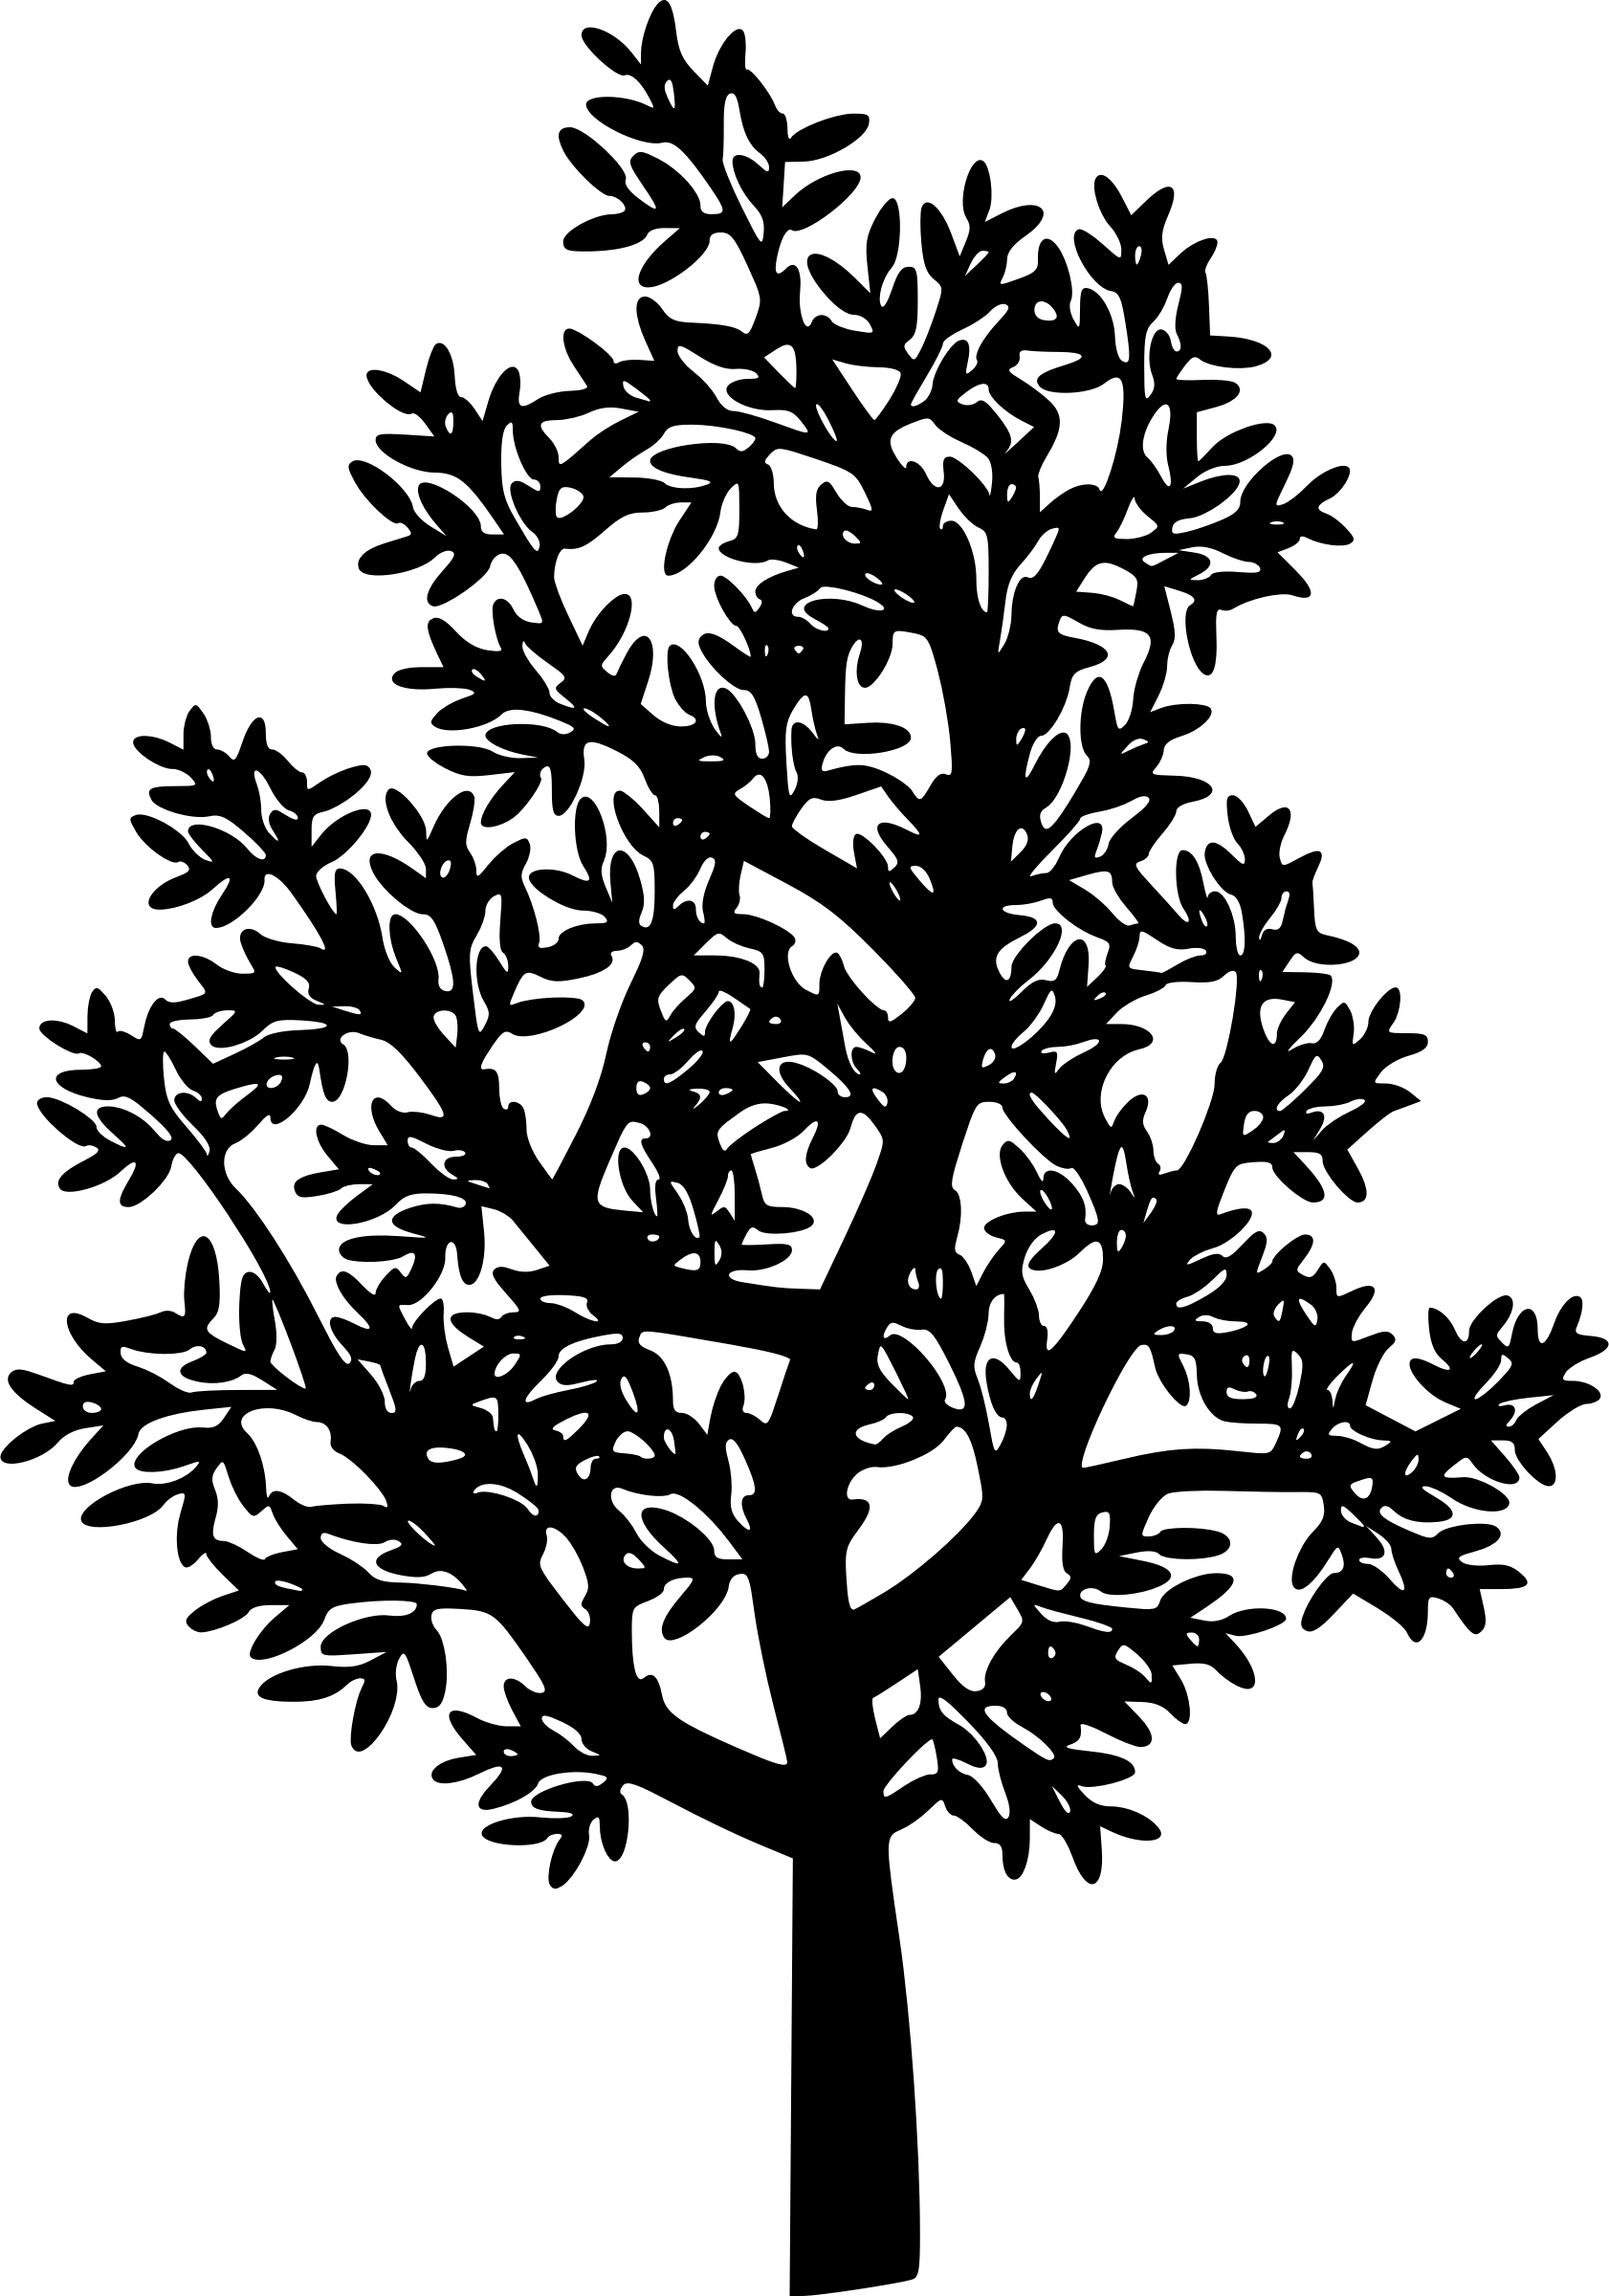
\includegraphics[width=.25in]{stuffs/tree3.png}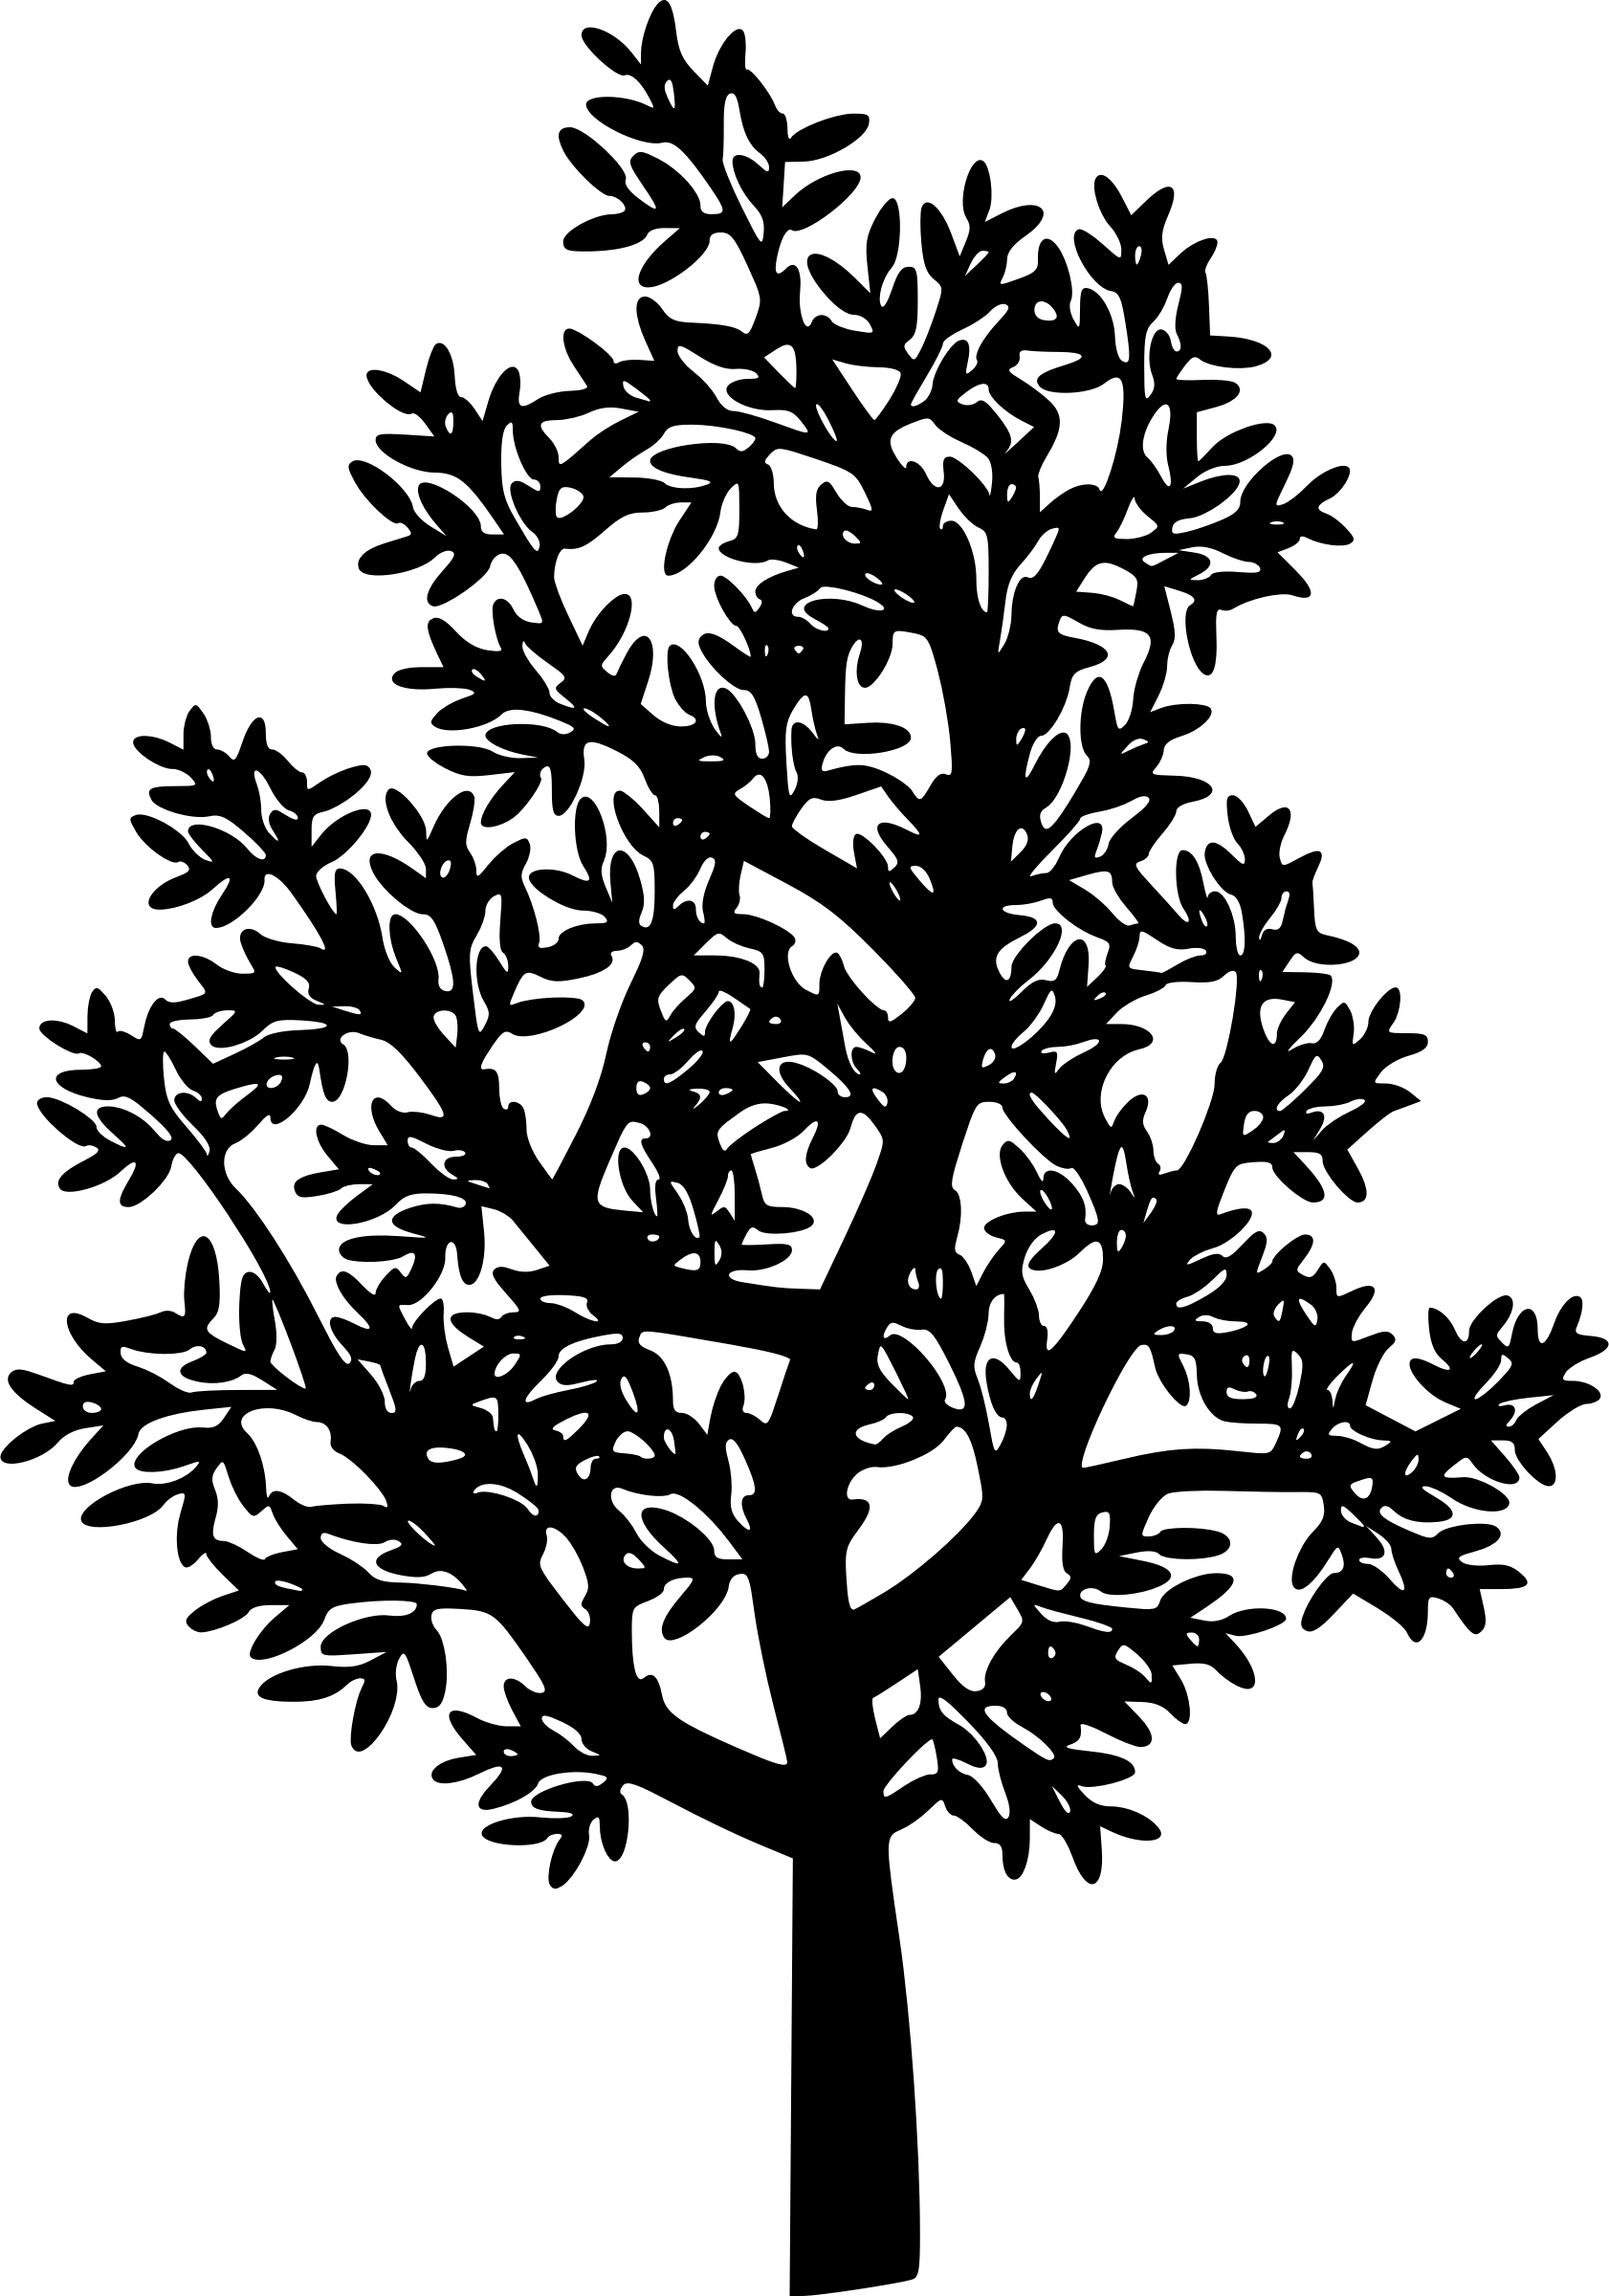
\includegraphics[width=.25in]{stuffs/tree3.png}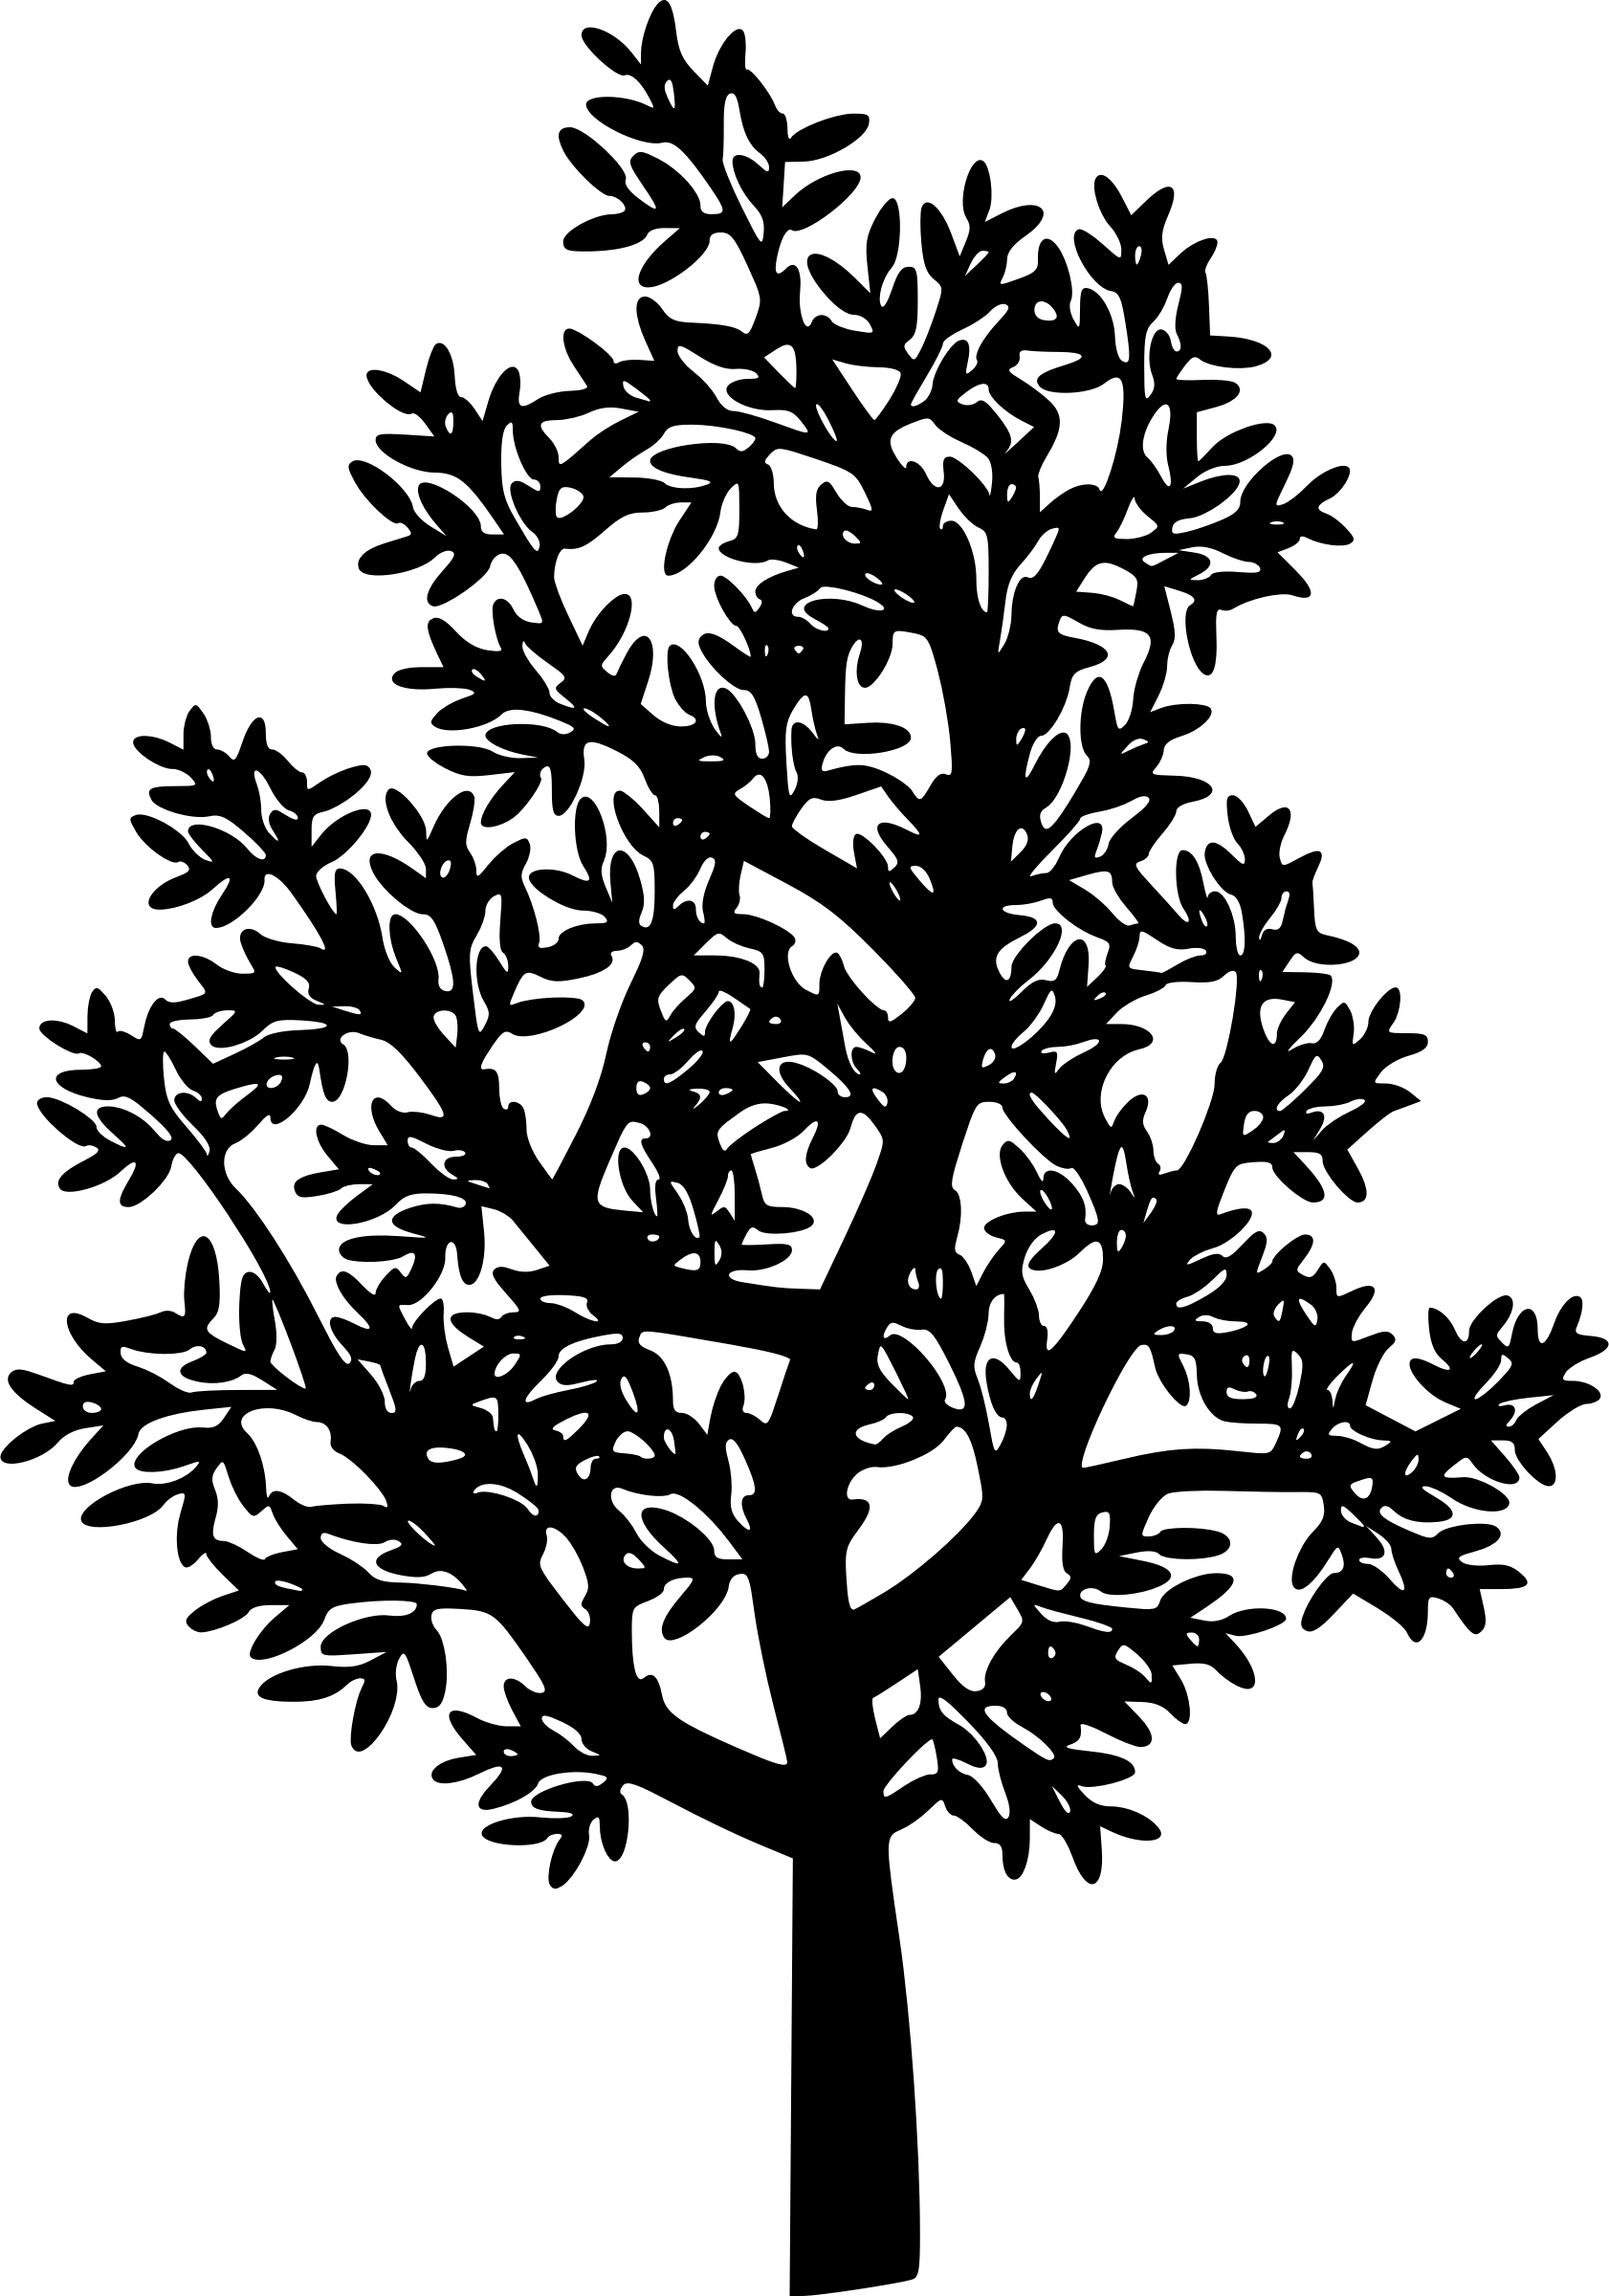
\includegraphics[width=.25in]{stuffs/tree3.png}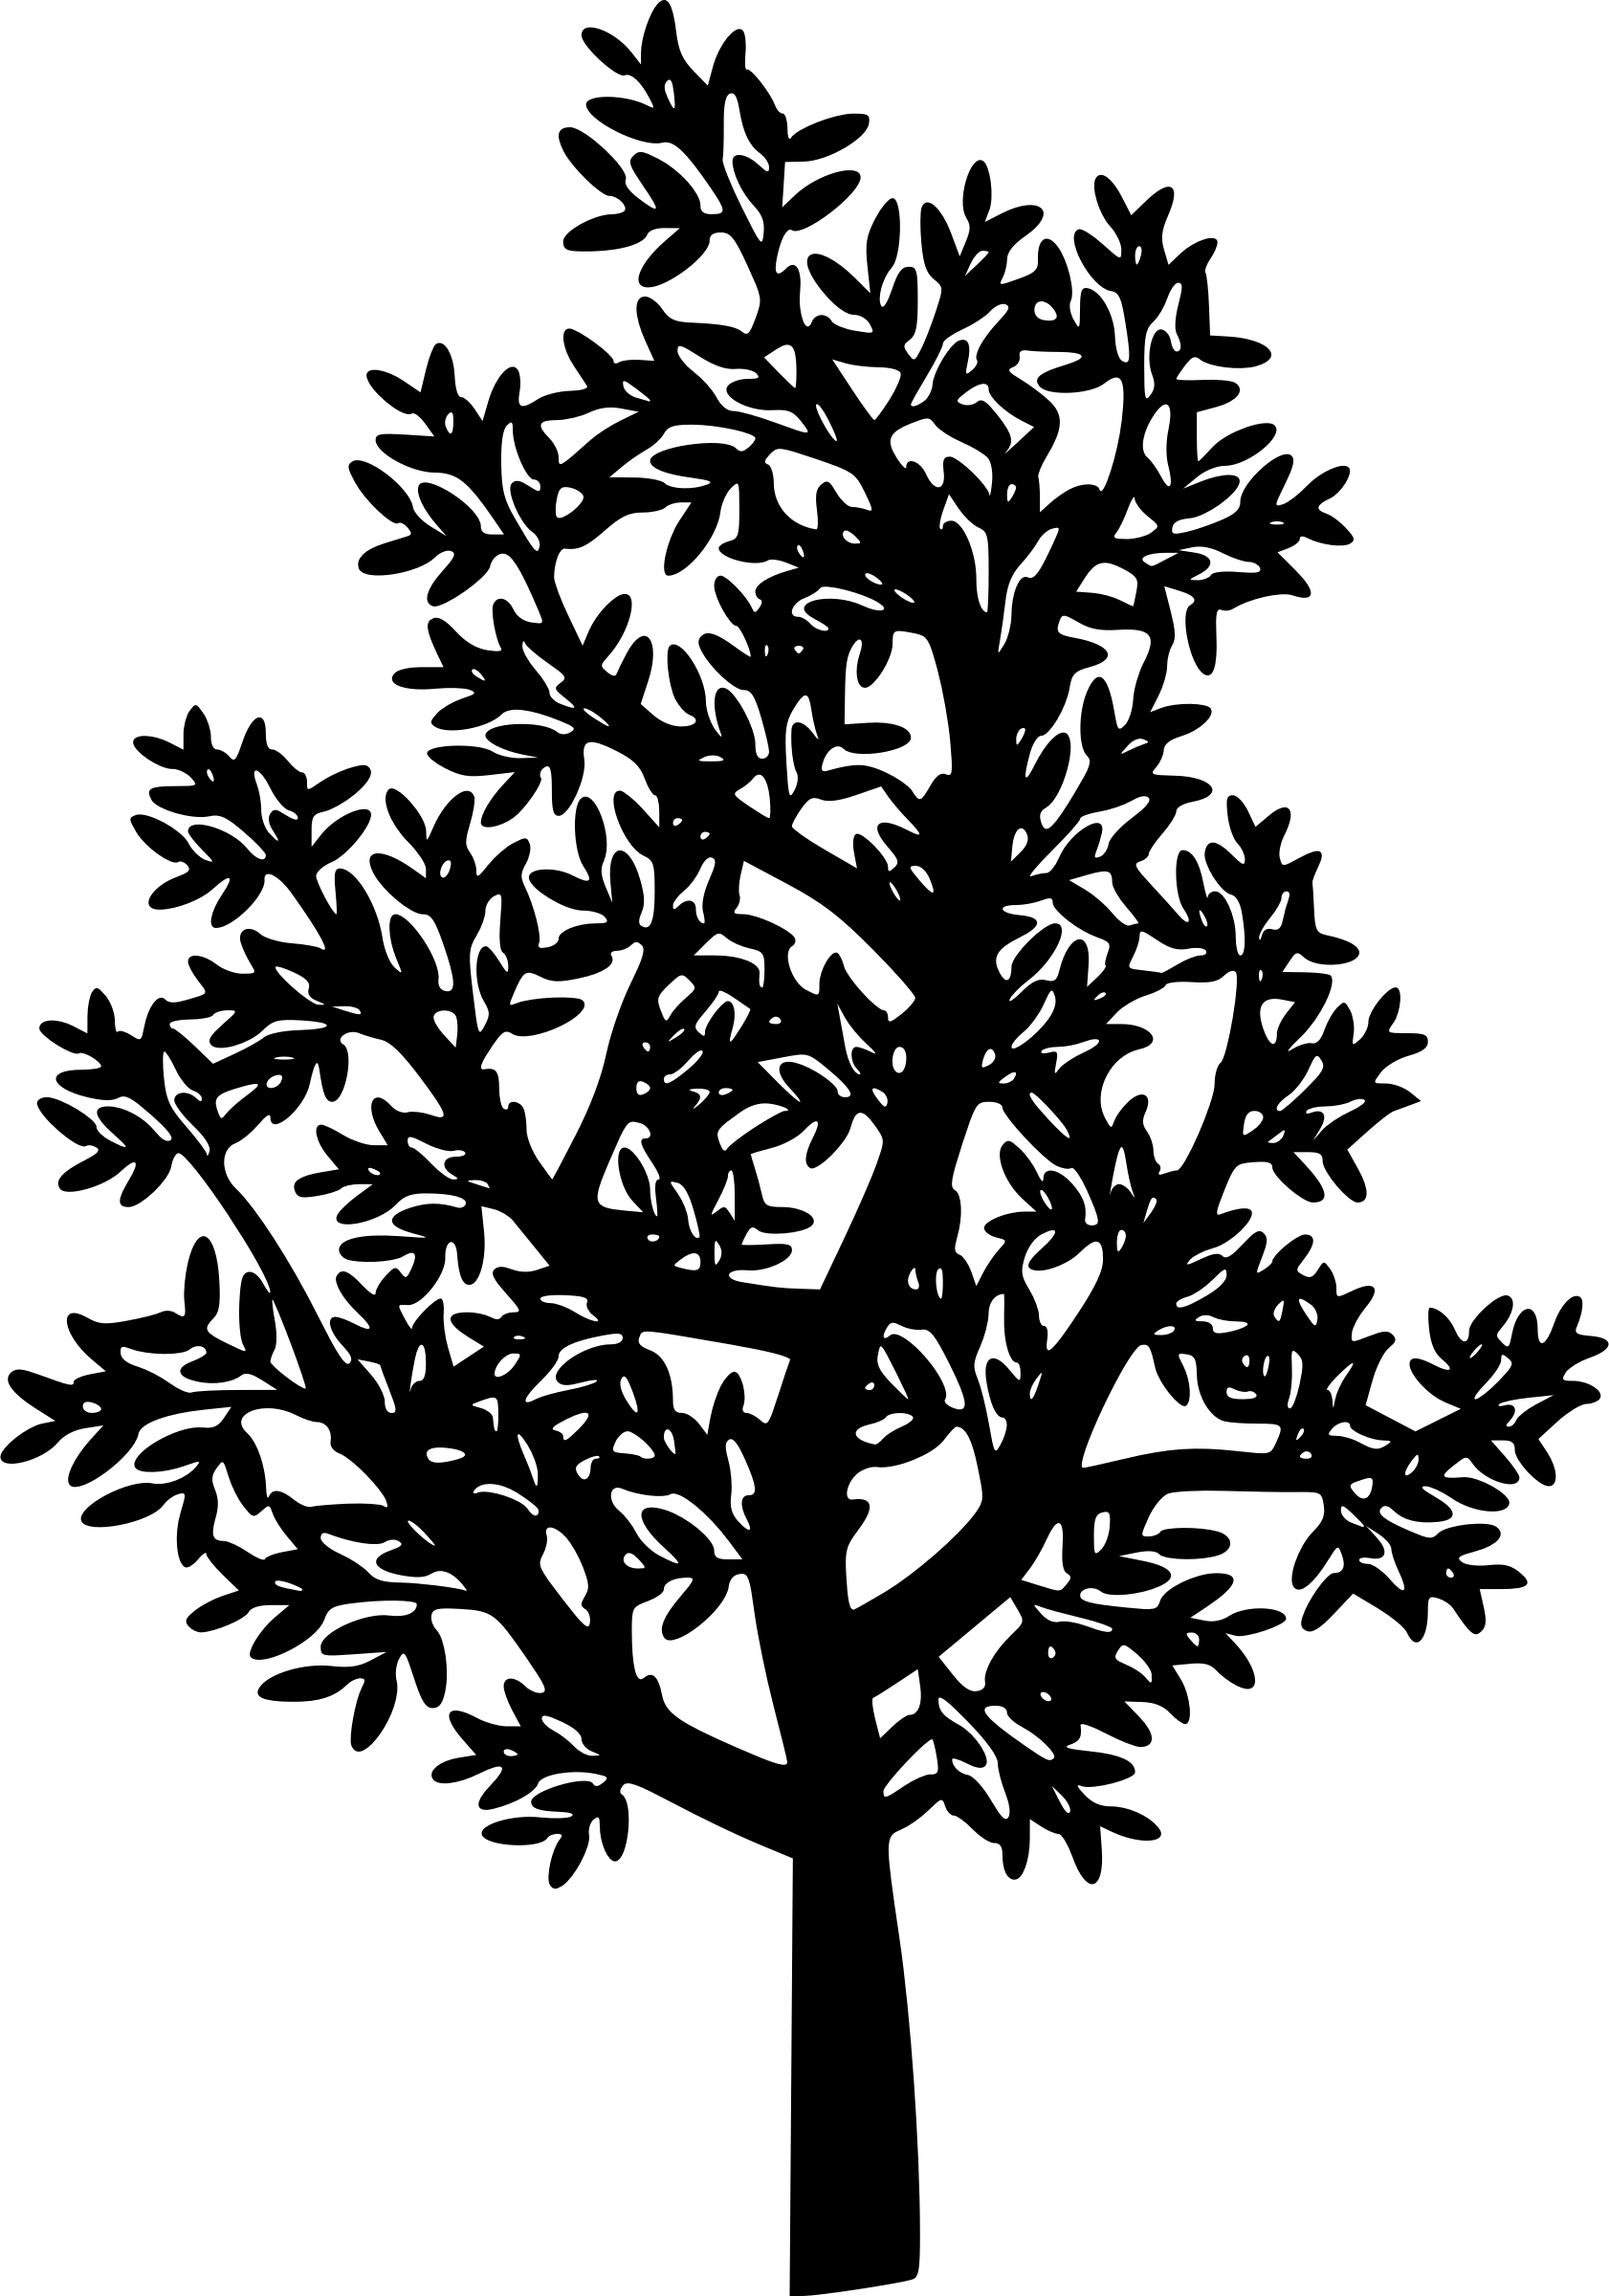
\includegraphics[width=.25in]{stuffs/tree3.png}\\${}$\\


\begin{enumerate}
\item[]<3-> \hspace{-2.25em} Trees are ``correlated'' because
\item<4->  bootstrap samples are about the same \textcolor{gray}{[nothing to do there]}
\item<5-> influential features tend to be same \textcolor{gray}{[this we could influence...]}
\item[]
\item[]<6-> \textcolor{red}{\emph{How can we make constructed tree not exactly the same? }}

\end{enumerate}

\end{column}
\begin{column}{.45\textwidth}

\onslide<2->{
\begin{figure}
\centering
\fbox{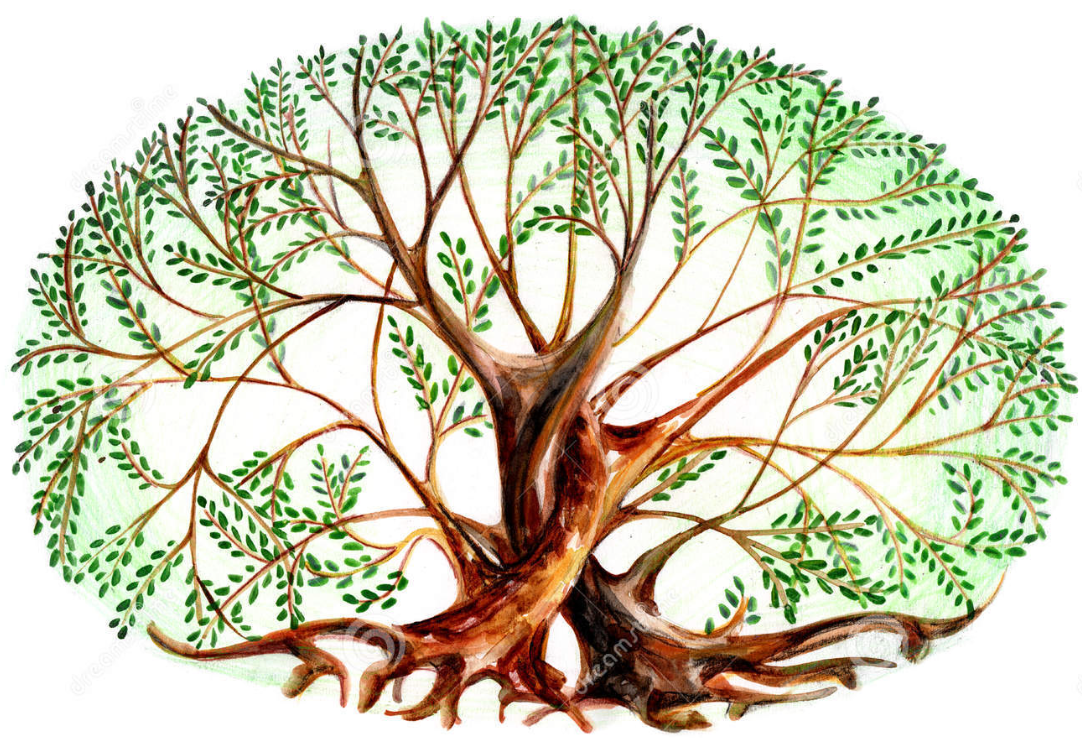
\includegraphics[width=1.55in]{stuffs/treeA.png}}

\Huge
$\Downarrow$

\vspace{.2em}

\fbox{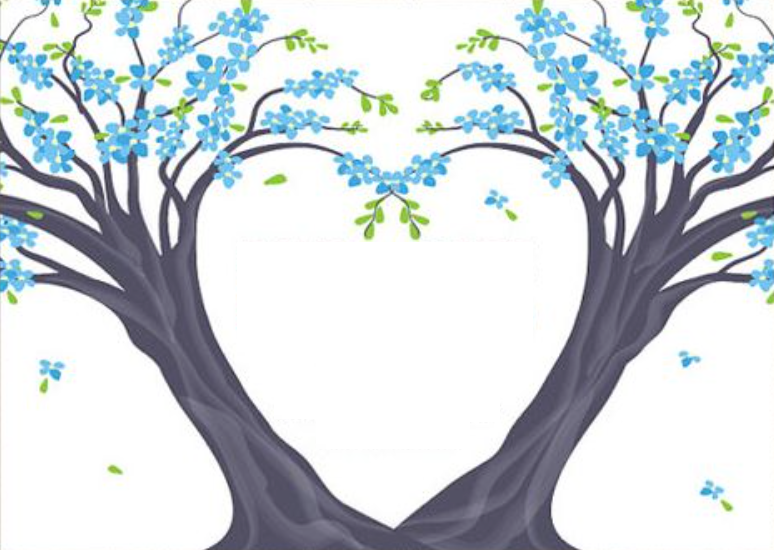
\includegraphics[width=1.55in]{stuffs/treeB.png}}
\end{figure}}

%\fbox{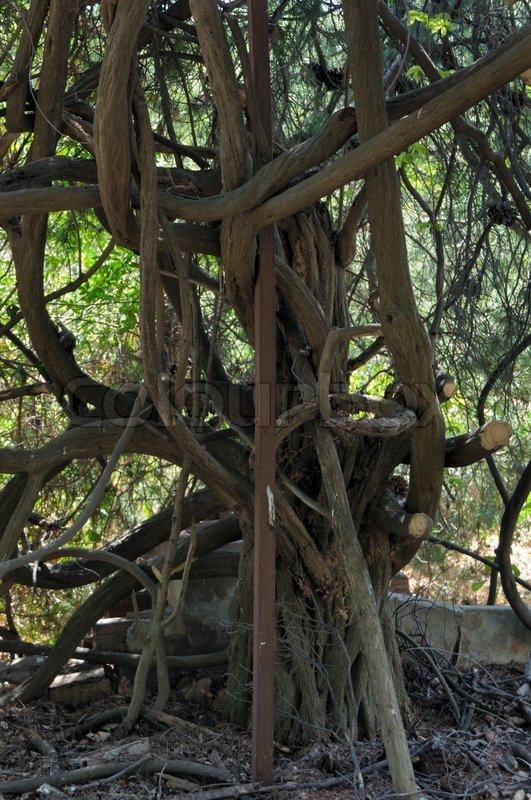
\includegraphics[width=1.75in]{tree2.jpg}}
\end{column}
\end{columns}

}

%\frame
%{
 %\frametitle{Favorite Joke!}
%\begin{figure}
%\centering
%\end{figure}
%}


\frame
{
\frametitle{Random Forests}


\begin{itemize}
\item<1-> Tree is constructed by recursive best splits
\item<3-> We only use a random subset of features \textbf{at each split}
\end{itemize}


\begin{columns}
\begin{column}{.5\textwidth}

\vspace{-.3in}

\begin{figure}
\centering

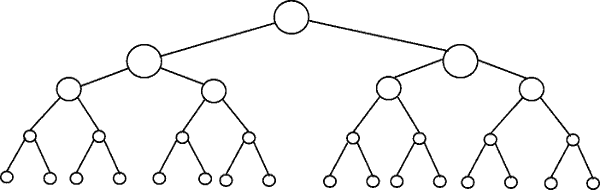
\includegraphics[width=2.3in]{stuffs/9XeYs.png}

\only<1>{\vspace{1.1in}}

\only<2>{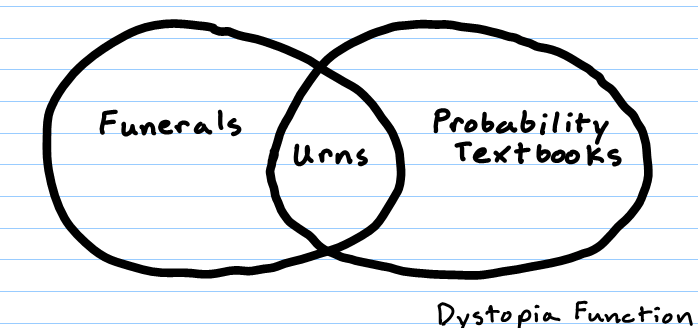
\includegraphics[width=2.3in]{stuffs/urns.PNG}}

\only<3>{${}$\\$\quad \txt{\die2 \die6}$\\${}$\\$\quad \;\spadesuit \; \square  \oslash  \oplus$
\vspace{.32in}
} 
\only<4->{${}$\\$\quad \txt{\die3 \die2}$\\${}$\\$\quad\clubsuit \; \blacksquare \otimes \odot$
\vspace{.32in}
}



\end{figure}

\end{column}
\begin{column}{.5\textwidth}

\begin{figure}
\centering
FEATURES

\begin{tabular}{|cccc|}
&&&\\
$\clubsuit$ & $\spadesuit$ & $\square$ & $\blacksquare$\\
 $\triangleleft$ & $\triangleright$ & $\triangledown$ & $\circ$\\
 $\Diamond$ & $\heartsuit$ & $\star$ & $\triangle$ \\
 $\oslash$ & $\oplus$ & $\odot$ & $\otimes$  \\ \hline
\end{tabular}
\begin{tabular}{c}
Features sampled with \\
replacement for possible \\
 use \textbf{at each node}  \\
\end{tabular}
\end{figure}
\end{column}
\end{columns}

\begin{itemize}
\item<5->  \underline{\emph{Temporary exclusion}} -- features includable again at each split
\item<6-> Typically select $\sqrt{p}$ (classification) \& $\frac{p}{3}$ (regression) features
\item<7->[] \textcolor{red}{Number features considered is a tuning parameter} for what?
\item<8-> \textcolor{blue}{More features  means stronger but also more correlated trees...} 
\end{itemize}

}




\frame
{
\frametitle{Random Forest \emph{Tuning}}

\begin{itemize}
\item<1->[$g(p)$:] Number of features considered at each split
\item<2->[$m$:] Number of trees \textcolor{gray}{(i.e., number of bootstrapped samples)}
\item<3->[$n_b$:] Sample size of each bootstrapped sample 
\item<4->[$\chi$:] Tree characteristics \onslide<5->{\textcolor{purple}{$\quad\quad\quad\quad\quad\Longrightarrow \sum ({\boldsymbol Y}_i - \hat {\boldsymbol Y}_i)^2 + \alpha |T|$}}
\end{itemize}
\vspace{-.5em}
\onslide<4->{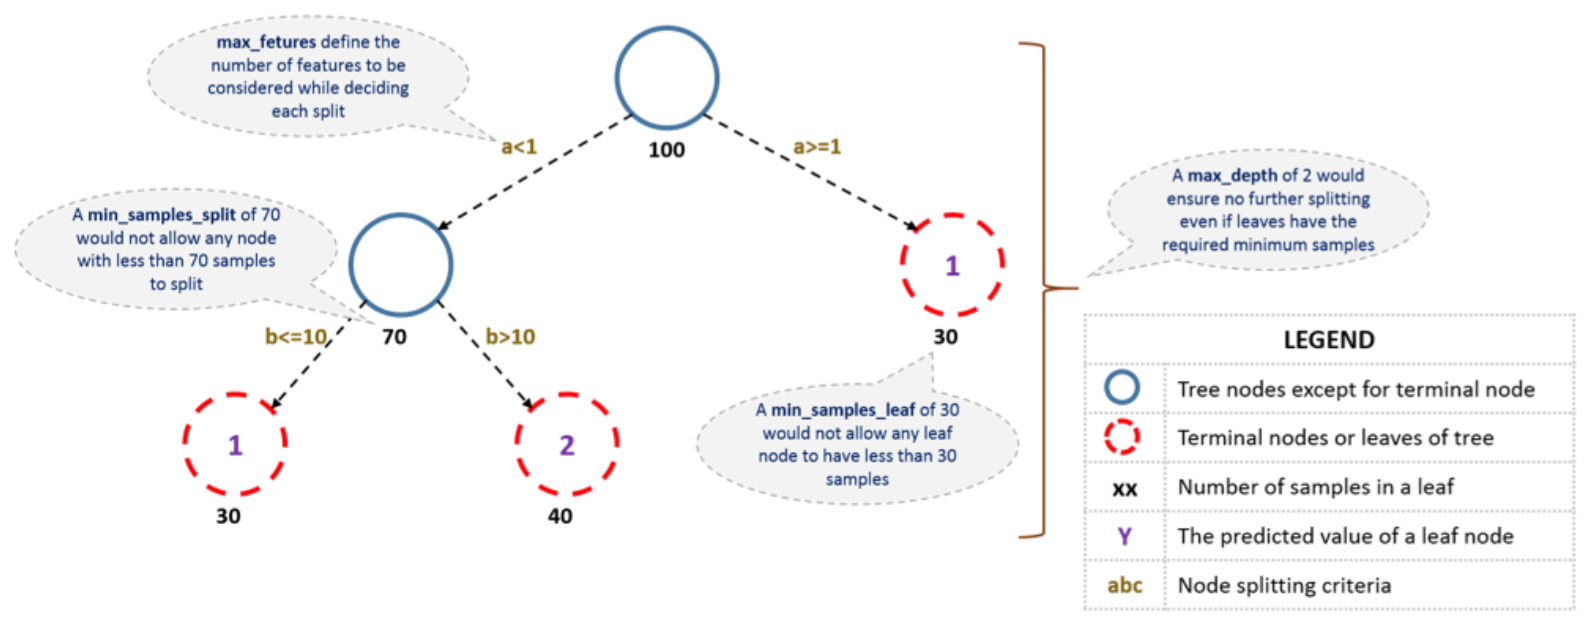
\includegraphics[width=4in]{stuffs/tunes.png}}
\vspace{-.5em}
\begin{itemize}
\item<6-> Random forests are often robust to tree characteristics:
\item<7->[] \textcolor{red}{\textbf{\emph{very large} numbers of ``bushy'' trees \underline{\emph{typically used}}} \&}  
% bushy and deep tree pruning is not needed -- we just use high variance predictor
\item<8->[] \textcolor{blue}{approach \textbf{\underline{state of the art} performance \underline{out of the box}}}

\end{itemize}
}

\frame
{
\frametitle{Random Forest \emph{Computational Notes}}

\begin{itemize}
\item<1-> Trees can be computationally expensive to fit
\begin{itemize}
\item<2-> But they can be fit in parallel 
\item<3-> At some point $\rho \sigma^2 \textcolor{gray}{+ (1 - \rho) \frac{\sigma^2}{m}}$ reaches an asymptote 
\item[]
\end{itemize}
\item<4-> Cross-validation can be computationally demanding
\item[]
\begin{itemize}
\item<5-> Parameters can be tuned using OOB\\${}$\\
\textcolor{red}{You have built-in test samples so you don't need K-folds --
you score a model right when it's fit at a specific tuning parameter!}\\${}$\\
\item<6-> Cross-validation is still needed for methodology comparisons...\\${}$\\
\textcolor{red}{OOB samples don't appear in other model fitting contexts -- so you still need a common ``out of sample" set to compare on...}
\end{itemize}
\end{itemize}
}




\frame
{
\frametitle{Interpreting Tree Ensembles}
${}$\\

``Plentie is nodeintie, ye see not your owne ease. I see, ye can not see the wood for trees.'' 
\begin{itemize}
\item[--] J. Heywood (1546) 
\item[]
\end{itemize}

 ``You can't see the forest for the treeeeeeees!''
\begin{itemize}
\item[--] M. Manson (1996)
\item[] 
\end{itemize}

\onslide<2->{
\noindent\makebox[\linewidth]{\rule{\paperwidth}{0.4pt}}

\begin{itemize}
\item[] 
\end{itemize}


``I find that people be all like, \footnotesize \\${}$

\textcolor{Maroon}{`Machine learning models are ``Black Boxes'' and you can't interpret them...',}\\${}$

\normalsize 
and I be like, \footnotesize \textcolor{NavyBlue}{`Damn you people have some back-ass wackwards ideas...'"}

\begin{itemize}
\item[--] S. Schwartz (Yesterday)
\item[] 
\end{itemize}


}

}



\frame
{
\frametitle{Interpreting Models}

\huge
Change $\boldsymbol X_i$ and see what happens\\${}$\\

\tiny It's just really not that hard...\LARGE \\${}$\\

\onslide<2->{
That's all your doing in a linear model: 

$$\beta_0 + \beta_1 X_1 + \beta_1 X_1 + \beta_2 X_2 + \cdots $$}

}





\frame
{
 \frametitle{Partial Dependency Plots}

\vspace{.6em}
\begin{enumerate}
\item<1-> Set feature $V=v$ for a single values $v$
\item<2-> Record average predictions $ \frac{1}{n} \sum_{i=1}^n \hat Y_i^{(v)}$ over  ``synthetic'' data 
\item<3-> Plot $\frac{1}{n} \sum_{i=1}^n \hat Y_i^{(v)}$ at $v$ \\ 
\end{enumerate}


\begin{figure}
\centering
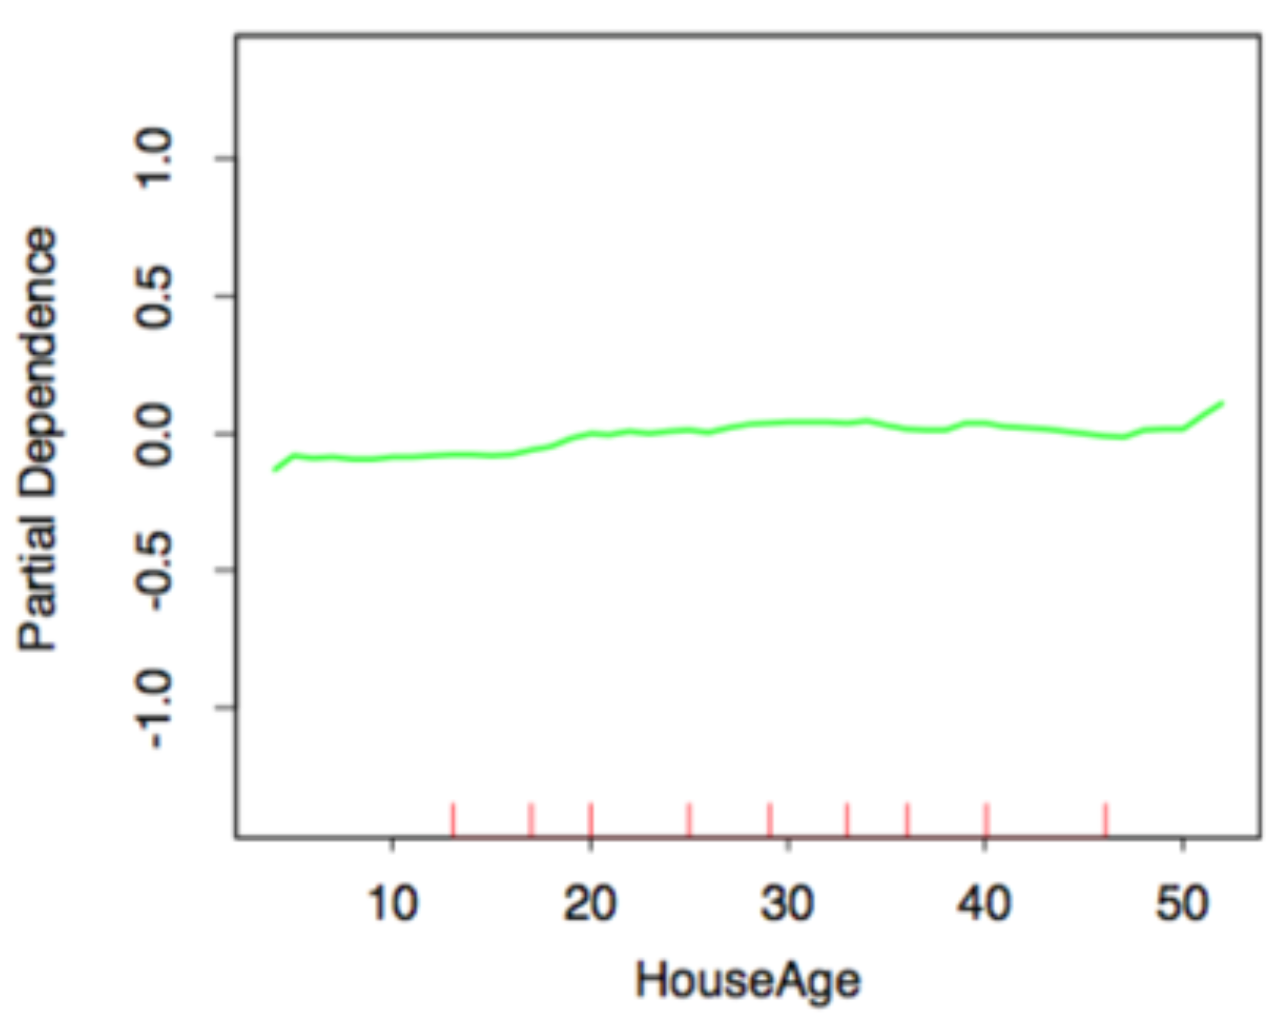
\includegraphics[width=1.5in]{stuffs/pd3.png}
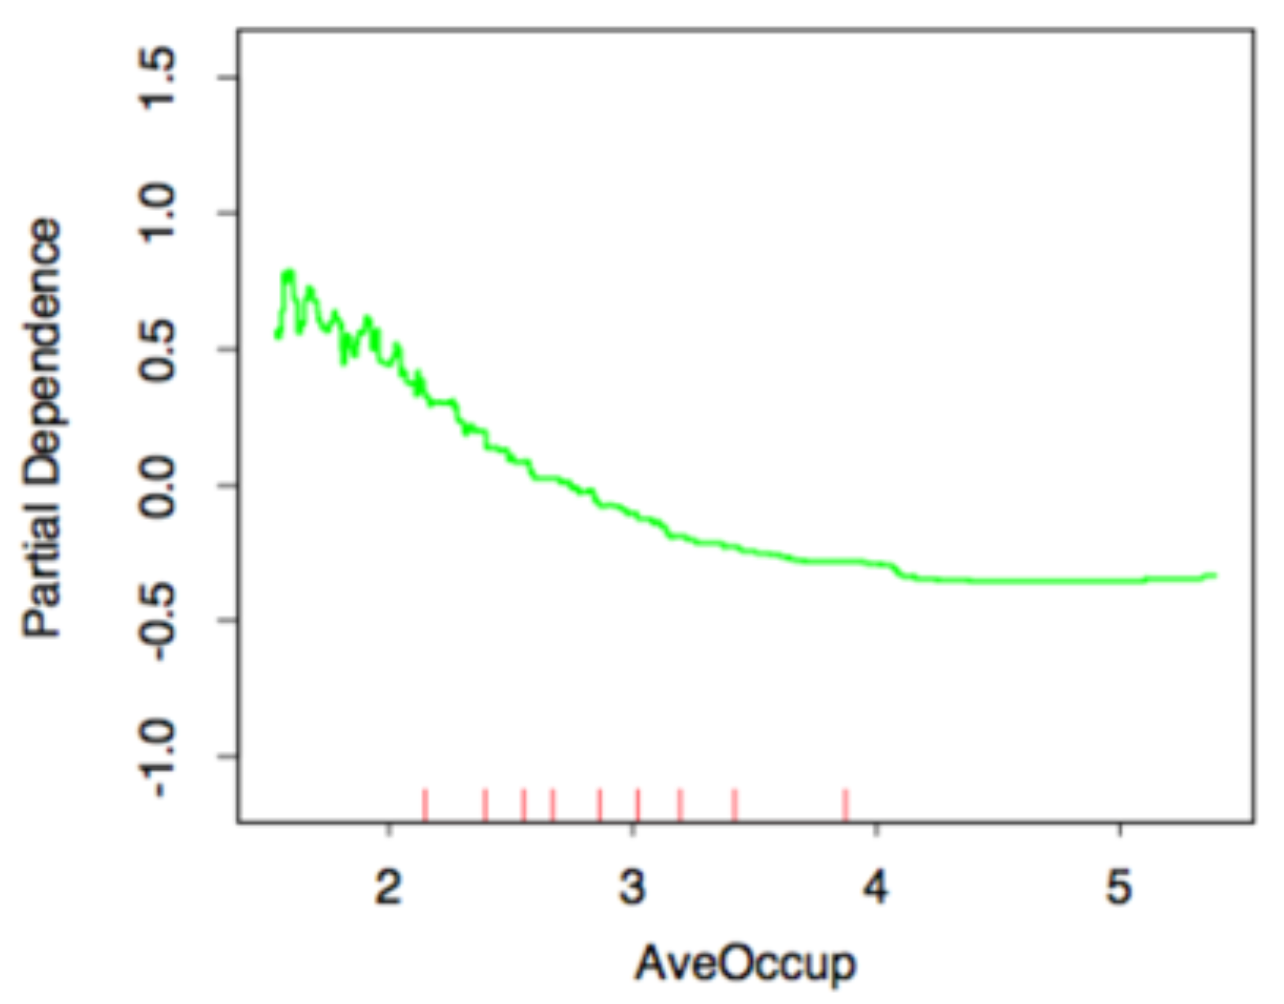
\includegraphics[width=1.5in]{stuffs/pd4.png}\\
\onslide<4->{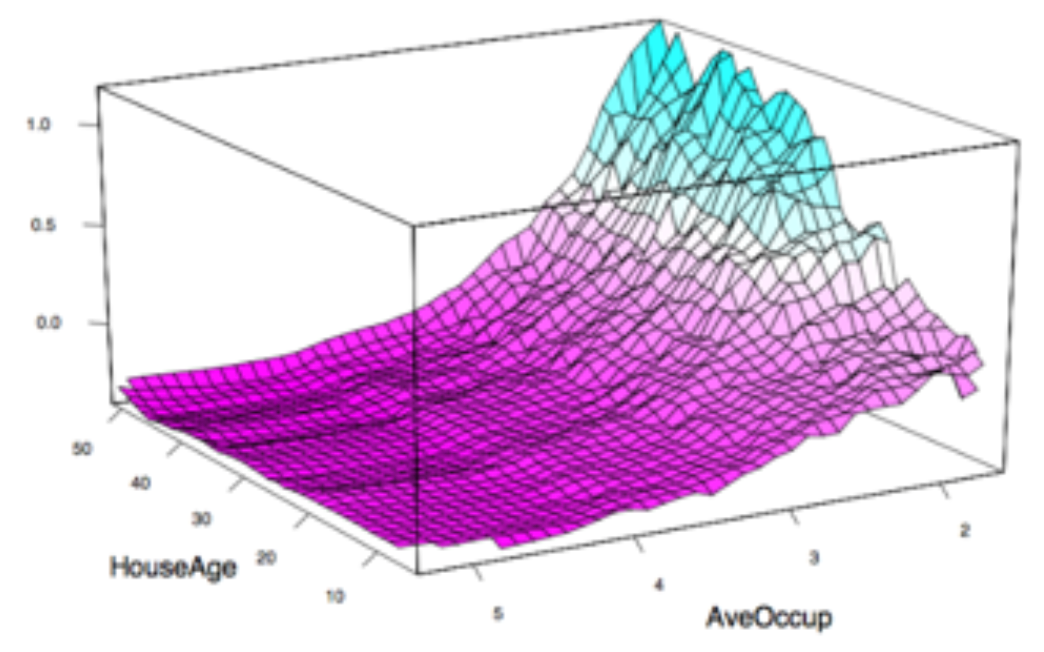
\includegraphics[width=2in]{stuffs/pd5.png}}
\end{figure}
}

\frame
{
 \frametitle{Variable Importance}

\huge
But there are some other \emph{Very Cool}
model interpretation options available in tree based contexts as well...

}


\frame
{
\frametitle{Variable Importance (v1.0): \textcolor{red}{``share of information gain''}}
\begin{enumerate}
\item<1-> Split are made on the feature minimizing RSS or Gini/Entropy
\item<2-> For split $s$, cumulate the explanatory contribution $\xi_V^{(s)}$ for $V$ 
\item<3-> Average the scores $\xi_V^{(s)}$ for each feature $V$ \textbf{across all trees}
\item[]<4->
\item[]<4->
\begin{figure}
\centering
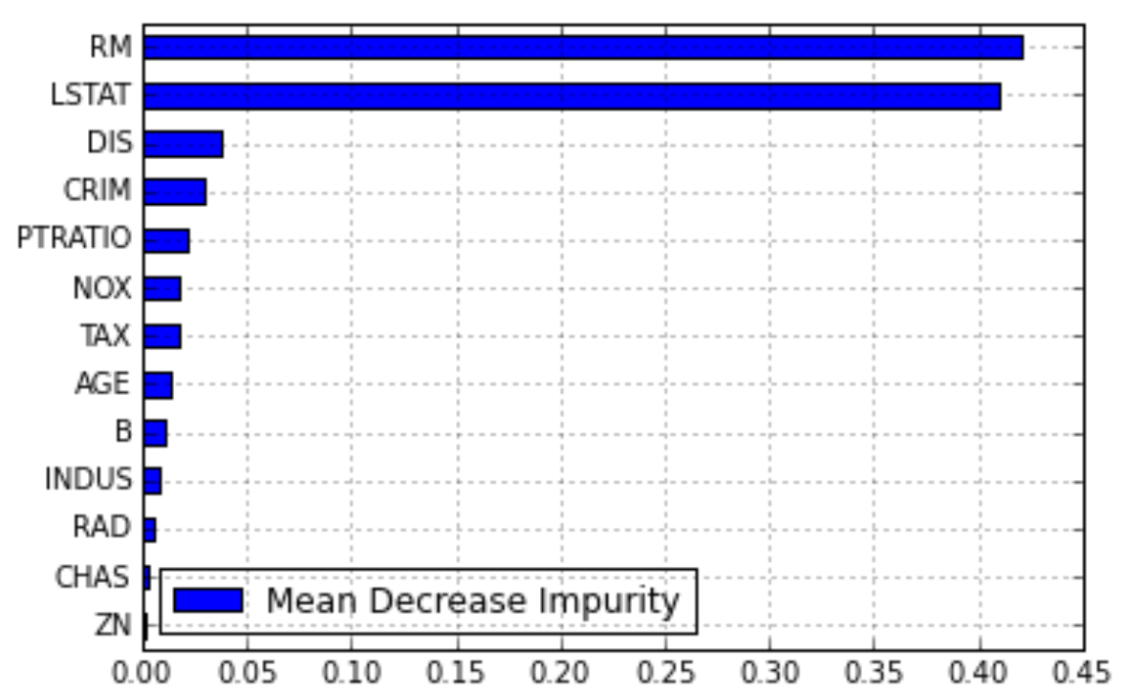
\includegraphics[width=2.75in]{stuffs/boston.png}

\footnotesize
\textcolor{gray}{
$\;\;\quad$In Boston, the most relevant associations with \\$\quad\;\;$neighborhood home values 
 are (1) number of rooms and \\$\;\;\quad$(2) proportion of low income households in the neighborhood }
\end{figure}

\end{enumerate}
}


\frame
{
\frametitle{Variable Importance (v2.0): \textcolor{red}{``error caused by losing $V$''}}
\begin{enumerate}
\item<1-> Get OOB accuracy using all features, including original $V$
\item<2-> Get OOB accuracy using all features \& $V^*$, a permuted $V$
\item<3-> Compare the differences between 1 and 2 for all features 
\item[]<3->% \emph{Results are predicted fitted on trees with $V$/$V^*$ and averaged}
% since individual trees are more sensitive than the random forest\\${}$\\
\item[]<4->
\begin{figure}
\centering
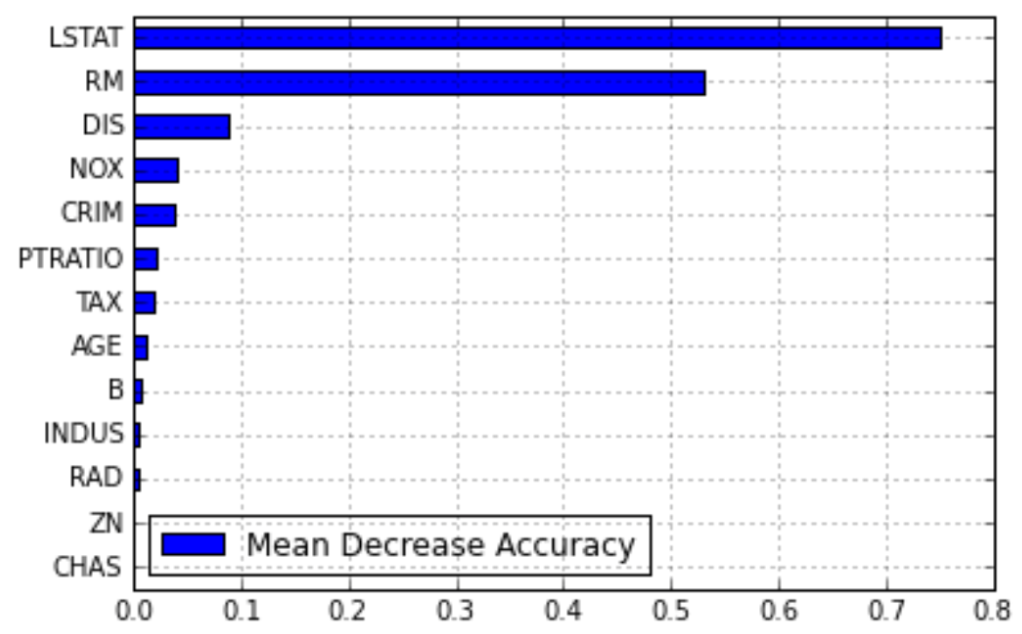
\includegraphics[width=2.75in]{stuffs/boston2.png}

\footnotesize
\textcolor{gray}{$\quad\;\;$This approach suggests prediction is more sensitive to \\$\quad\;\;$(1)  low income proportion rather than (2) room number}

\end{figure}
\end{enumerate}
}



\frame
{
\frametitle{Variable Importance (v3.0): \textcolor{red}{``what influences predictions''}}
\begin{enumerate}
\item<1-> Follow test samples down the tree through each split $s$ on $V$
\item<2-> Record the change in prediction $\epsilon^{(s)}_V$ due to $V$ split at $s$ 
\item<3-> Sum up all the changes $\epsilon^{(s)}_V$ due to feature $V$
\item[]<4-> \emph{These values are then averaged across trees}
% since individual trees are more sensitive than the random forest\\${}$\\
\item[]<5->
\begin{figure}
\centering
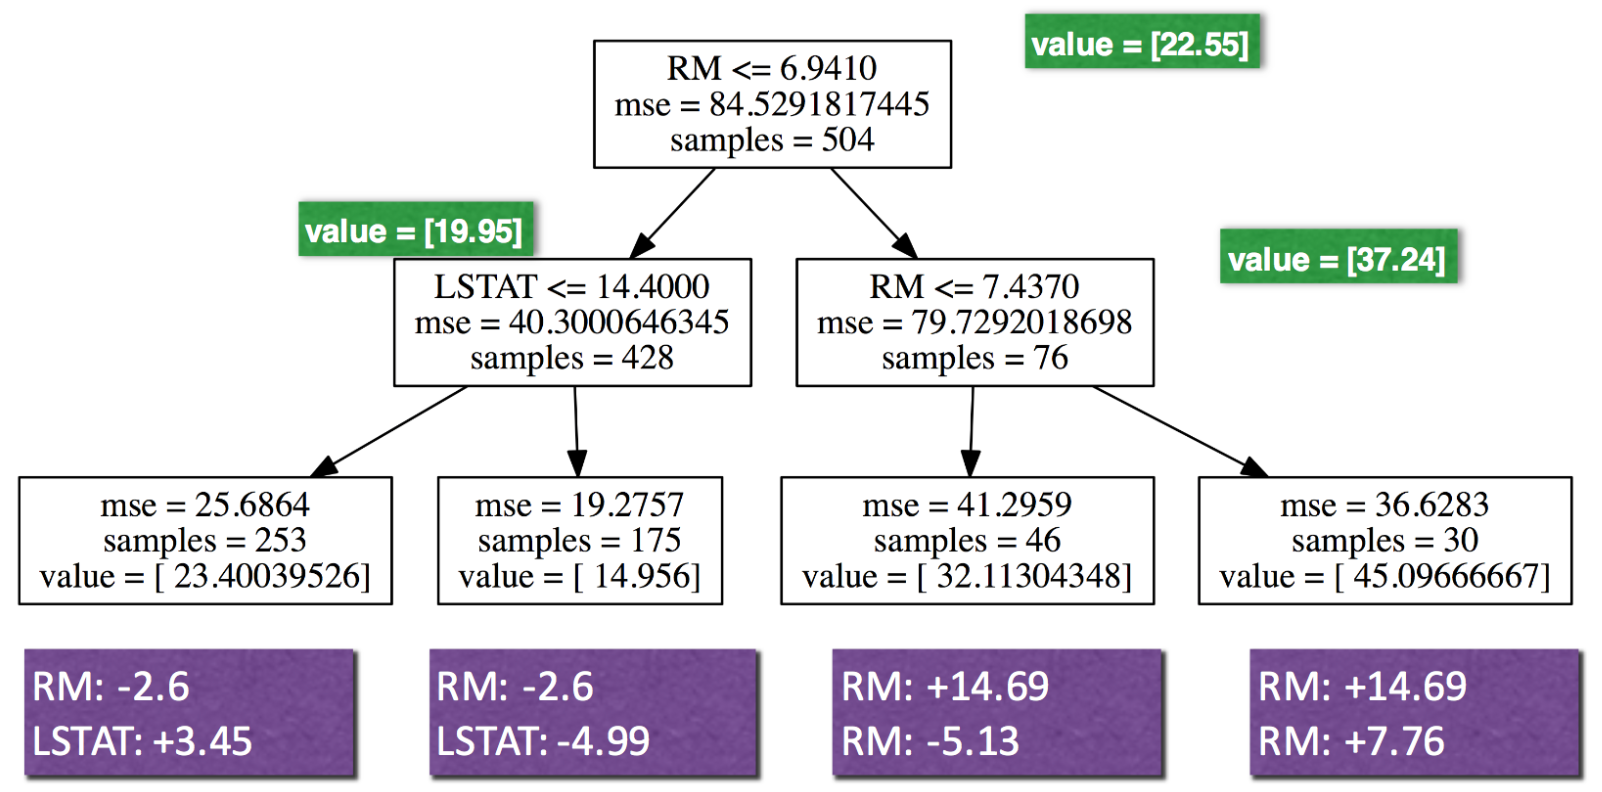
\includegraphics[height=1.955in]{stuffs/flow.png}
\end{figure}
\end{enumerate}
}

\frame
{
\frametitle{Variable Importance (v3.0): \textcolor{red}{``what influences predictions''}}
\begin{enumerate}
\item Follow test samples down the tree through each split $s$ on $V$
\item Record the change in prediction $\epsilon^{(s)}_V$ due to $V$ split at $s$ 
\item Sum up all the changes $\epsilon^{(s)}_V$ due to feature $V$
\item[] \emph{These values are then averaged by tree}
% since individual trees are more sensitive than the random forest\\${}$\\
\item[]
\begin{figure}
\centering %2.12
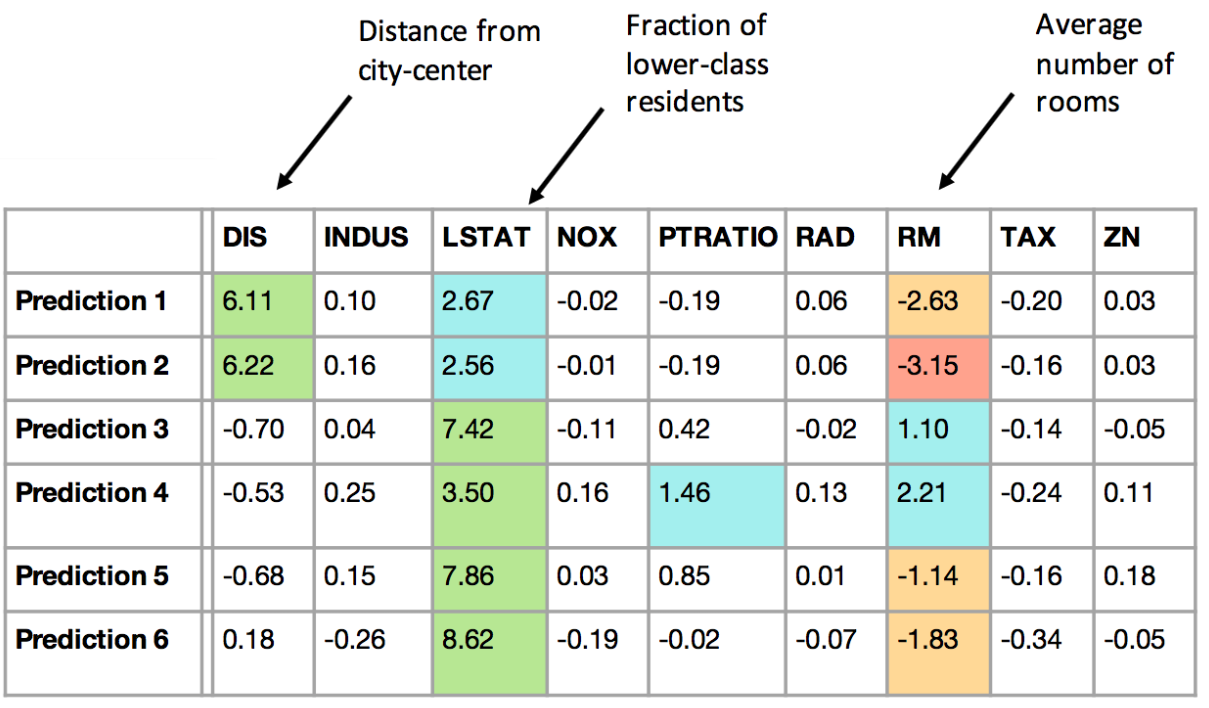
\includegraphics[height=1.89in]{stuffs/flow2.png}\\
\textcolor{red}{Features effects can be characterized on individual samples (!)}% (cool)
\end{figure}
\end{enumerate}
}


\frame
{
\frametitle{Variable Importance (v4.0): \textcolor{red}{``what the tree predicts with''}}

\begin{enumerate}
\item<1-> Calculate proportion of samples visiting feature $V$ in each tree
\item<2->[] (conditions higher in the tree typically visited by more data) 
\item<3-> Average the ``proportion of samples visited''  across all trees

\vspace{2.45in}
\end{enumerate}

}



\frame
{
\frametitle{Fine}


So don't tell me machine learning models, \emph{particularly tree-based methods} are uninterpretable ``Black-Boxes''. I'll kick your butt.\\${}$\\${}$\\${}$\\${}$\\

\onslide<2->{
Now: 

\begin{figure}
\centering
\Large
\textbf{Tree $<$ Bagging $<$ Random Forests $<$ \underline{$\quad\quad\quad$?}}
\end{figure}
}}


\end{document} 




\frame
{
 \frametitle{Partial Dependency Plots}

\hspace*{-.8cm}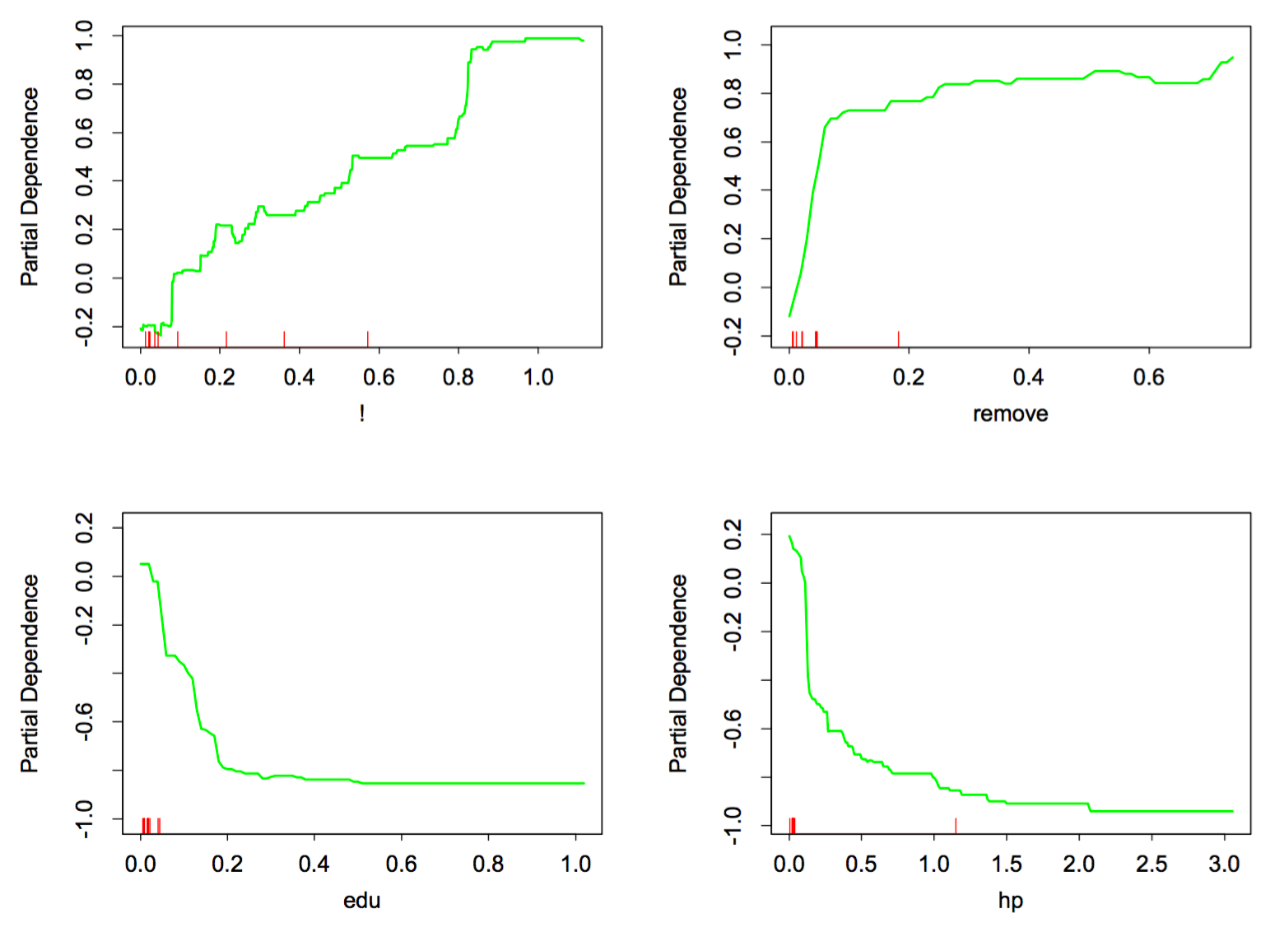
\includegraphics[width=2.3in]{stuffs/pd2.png}\raisebox{-1em}{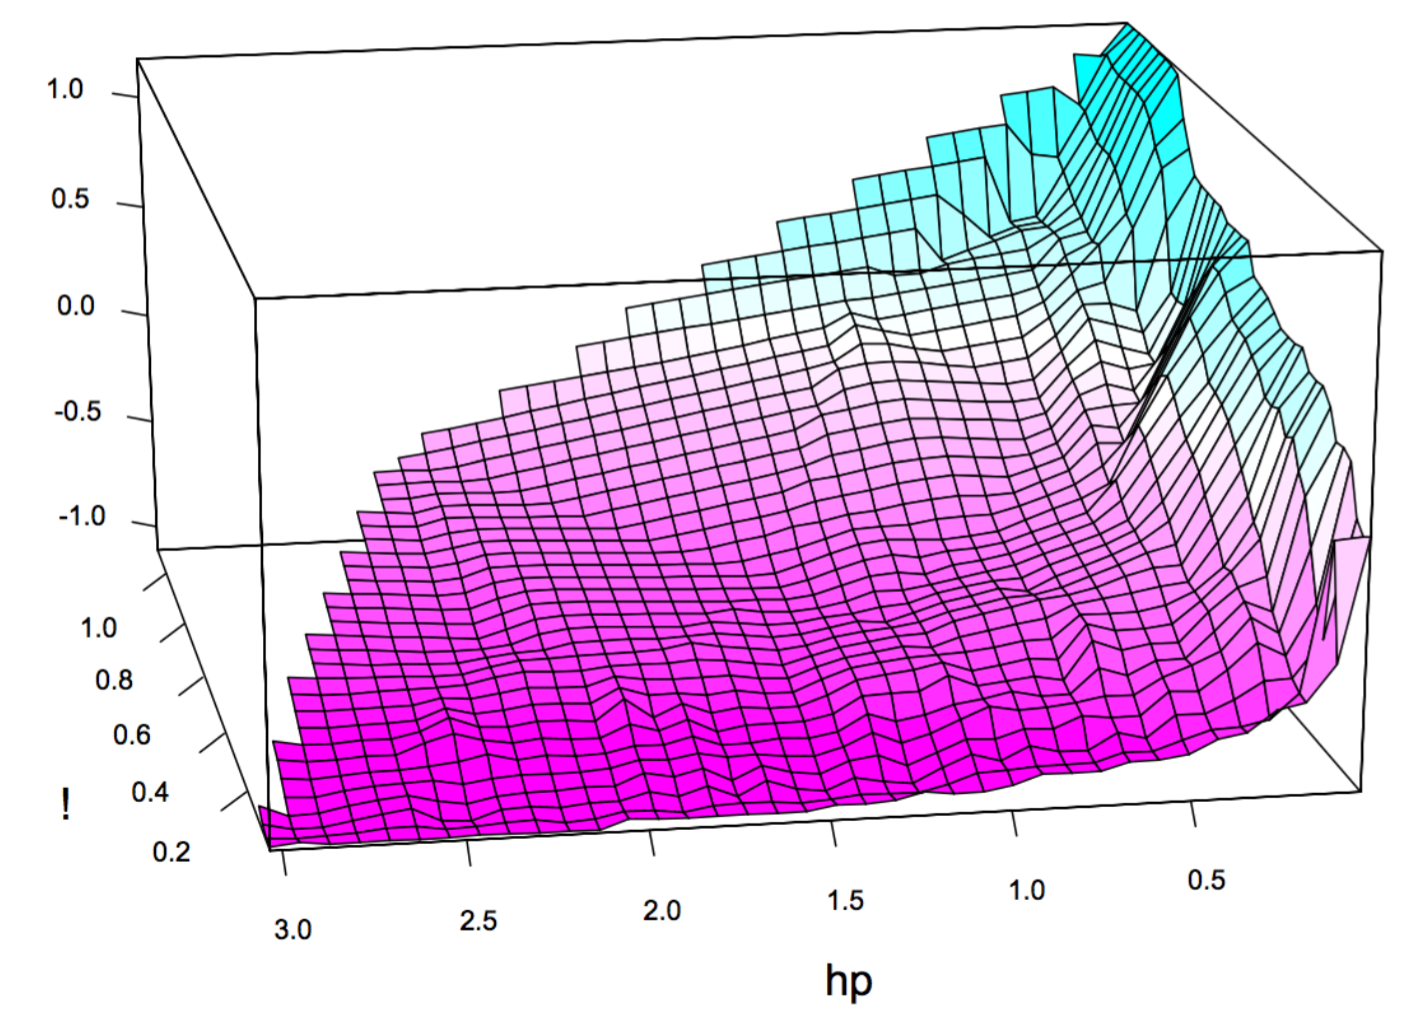
\includegraphics[width=2.6in]{stuffs/pd1.png}}

}






